% !TEX options=--shell-escape
\documentclass[usenames,dvipsnames,9pt]{beamer}

\usepackage{tikz}
\usetikzlibrary{arrows,shapes,snakes,automata,calc,matrix,backgrounds,petri, positioning}

\makeatletter
\def\input@path{{support/beamer-template/}}
\makeatother

\usepackage{support/beamer-template/beamerthememetropolis}

\usepackage[utf8]{inputenc}
\usepackage[czech]{babel}
\selectlanguage{czech}

\usepackage{hyperref}
\usepackage{fontawesome}
\usepackage{minted}
\usepackage{mathtools}
\usepackage{tabularx}
\usepackage{smartdiagram}
\usepackage{soul}
\usepackage{tikz}
\usepackage{amssymb}
\usepackage{qrcode}

% Commands shared between most of the tutorial slides

% Homework deadlines
\newcommand{\hwVIIdeadline}{10. 5. 2020}



% Download icon and text with link relative to the root of the courseware site
\newcommand{\download}[1]{\hfill\faDownload\hspace{5pt}\href{https://cw.fel.cvut.cz/wiki/_media/courses/be4m36mas/#1}{\tt #1}\\[1.3em]}

% Draw eye icon
\newcommand{\see}[1]{\faEye\hspace{5pt}#1}

\newcommand{\sep}{\hspace{10pt}/\hspace{10pt}}

\def\Ipe#1{\def\IPEfile{#1}\input{#1}}

% Draw pacman icon
\newcommand{\pacman}[1]{\tikz[baseline=.1em,scale=.6]{
    \useasboundingbox (.02,0) rectangle (.6,.6);
  \draw [fill=#1] (.3,.3) -- ++(25:.3) arc (+25:+335:.3) -- cycle;

}}

% Draw ghost icon
\newcommand{\ghost}[1]{\tikz[baseline=.1em,scale=.5]{
  \draw [fill=#1] (0,0) -- (0,.5) arc (+180:0:.3) -- (.6,0) --
  (.5,.15) -- (.4,0) -- (.3,.15) -- (.2,0) -- (.1,.15) -- cycle;
    \coordinate (eye) at (360*rand:.03);
    \foreach \x in {.17,.43}{
      \fill[white] (\x,.5) circle[radius=.1];
      \fill[black] (\x,.5) ++(eye) circle[radius=.05];
    }
}}

\newcommand{\desc}[2]{
  #1

  \vspace{-0.6em}
  \hfill\begin{minipage}{0.9\linewidth}
    #2
  \end{minipage}

  \vspace{0.2em}
}

\newcommand{\redc}{\tikz\draw[red,fill=red] (0,0) circle (.5ex);}

\newcommand{\greenc}{\tikz\draw[green,fill=green] (0,0) circle (.5ex);}


% Default url for generating QR code with feedback form.
\newcommand{\defaultfeedbackurl}{https://forms.gle/vwbWazEu14w1Kf487}

% Generate frame with QR code to a feedback form.
\newcommand{\framefeedback}[1][\defaultfeedbackurl]{
  \begin{frame}[standout]
    \begin{minipage}{0.4\linewidth}
      \begin{center}
        \textbf{\LARGE Díky za pozornost!}
      \end{center}

      \vspace{3em}

      \raggedleft\small Budeme rádi za Vaši\\zpětnou vazbu! $\rightarrow$
    \end{minipage}
    \hfill
    \begin{minipage}{0.5\linewidth}
      \vspace{4em}
      \centering\qrcode[height=\linewidth]{#1}\\
      \vspace{0.8em}
      \url{#1}
    \end{minipage}
  \end{frame}
}

%
% \newcommand{\download}[1]{\hfill\faDownload\hspace{5pt}\href{https://cw.fel.cvut.cz/wiki/_media/courses/be4m36mas/#1}{\tt #1}\\[1.3em]}
% \newcommand{\see}[1]{\faEye\hspace{5pt}#1}
% \newcommand{\sep}{\hspace{10pt}/\hspace{10pt}}
% \def\Ipe#1{\def\IPEfile{#1}\input{#1}}
%
% \newcommand{\pacman}[1]{\tikz[baseline=.1em,scale=.6]{
%     \useasboundingbox (.02,0) rectangle (.6,.6);
%   \draw [fill=#1] (.3,.3) -- ++(25:.3) arc (+25:+335:.3) -- cycle;
%
% }}
%
% \newcommand{\ghost}[1]{\tikz[baseline=.1em,scale=.5]{
%   \draw [fill=#1] (0,0) -- (0,.5) arc (+180:0:.3) -- (.6,0) --
%   (.5,.15) -- (.4,0) -- (.3,.15) -- (.2,0) -- (.1,.15) -- cycle;
%     \coordinate (eye) at (360*rand:.03);
%     \foreach \x in {.17,.43}{
%       \fill[white] (\x,.5) circle[radius=.1];
%       \fill[black] (\x,.5) ++(eye) circle[radius=.05];
%     }
% }}
%
%
% \newcommand{\desc}[2]{
%   #1
%
%   \vspace{-0.6em}
%   \hfill\begin{minipage}{0.9\linewidth}
%     #2
%   \end{minipage}
%
%   \vspace{0.2em}
% }
%
% \newcommand{\redc}{\tikz\draw[red,fill=red] (0,0) circle (.5ex);}
% \newcommand{\greenc}{\tikz\draw[green,fill=green] (0,0) circle (.5ex);}

\title{Čas a detekce selhání v distribuovaných systémech}
\date{}
\institute{B4B36PDV -- Paralelní a distribuované výpočty}

\metroset{block=fill}

\begin{document}
\maketitle

\begin{frame}
  \frametitle{Osnova}
  \begin{itemize}
    \item Opakování z minulého cvičení\\[1.5em]
    \item Detekce selhání v distribuovaných systémech
    \item Čas a uspořádání událostí v distribuovaných systémech\\[1.5em]
    \item Zadání 6. domácí úlohy
  \end{itemize}
\end{frame}

\begin{frame}[standout]
  \begin{minipage}{0.4\linewidth}
    \begin{center}
      \textbf{\LARGE Odevzdání semestrální práce se blíží!}
    \end{center}

    \vspace{3em}

    \begin{center}
      \textbf{Neděle 7.5. 23:59 CET}
    \end{center}

    %\raggedleft\small Budeme rádi za Vaši\\zpětnou vazbu! $\rightarrow$
  \end{minipage}
  \hfill
  \begin{minipage}{0.5\linewidth}
    \vspace{.3em}
    \centering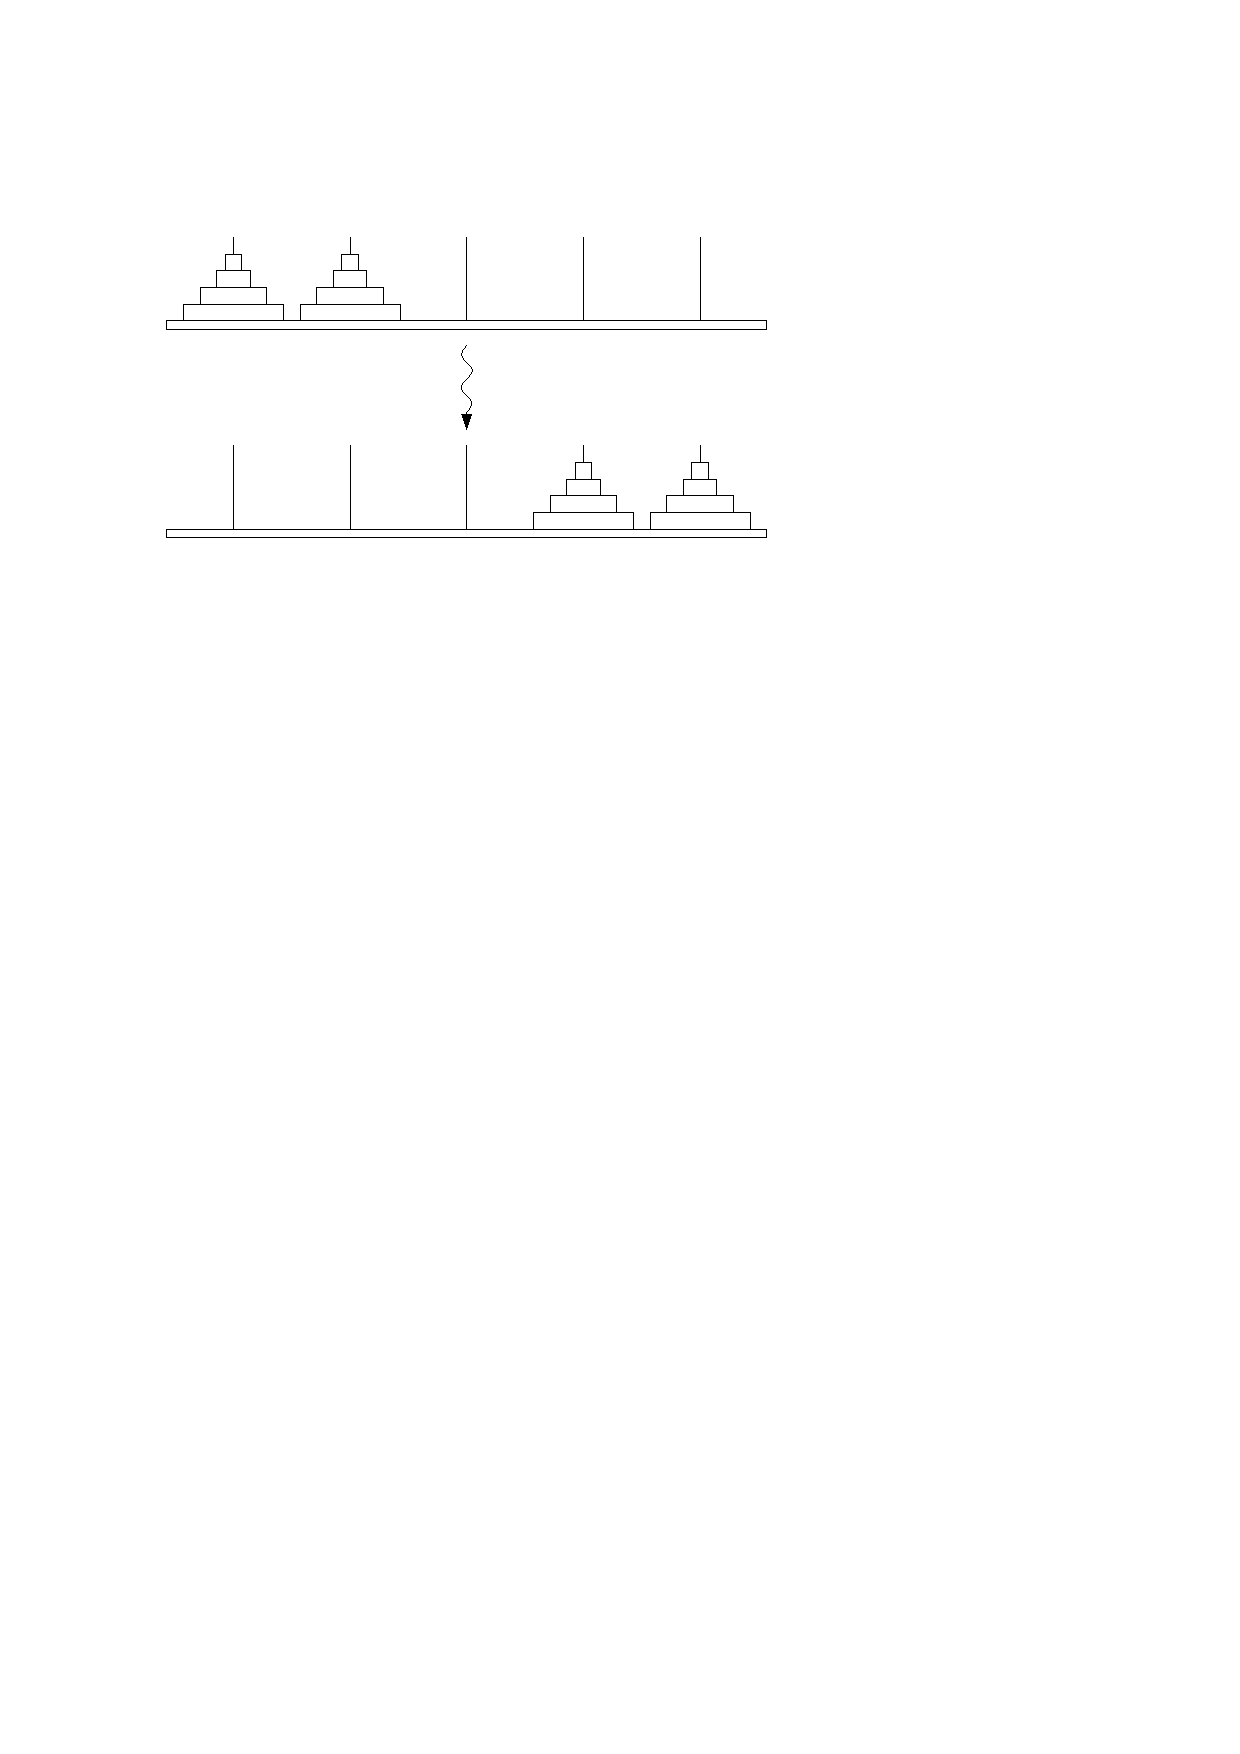
\includegraphics[width=\linewidth]{10/figs/hanoi.pdf}

    %\raggedleft\url{https://goo.gl/forms/CQGculehxhM8TwVq2}
  \end{minipage}

  \vspace{3em}



\end{frame}


\section{Opakování z minulého cvičení}

\begin{frame}[standout]
 \Huge
 \url{http://goo.gl/a6BEMb}
\end{frame}

\begin{frame}
\frametitle{DSand framework}
\centering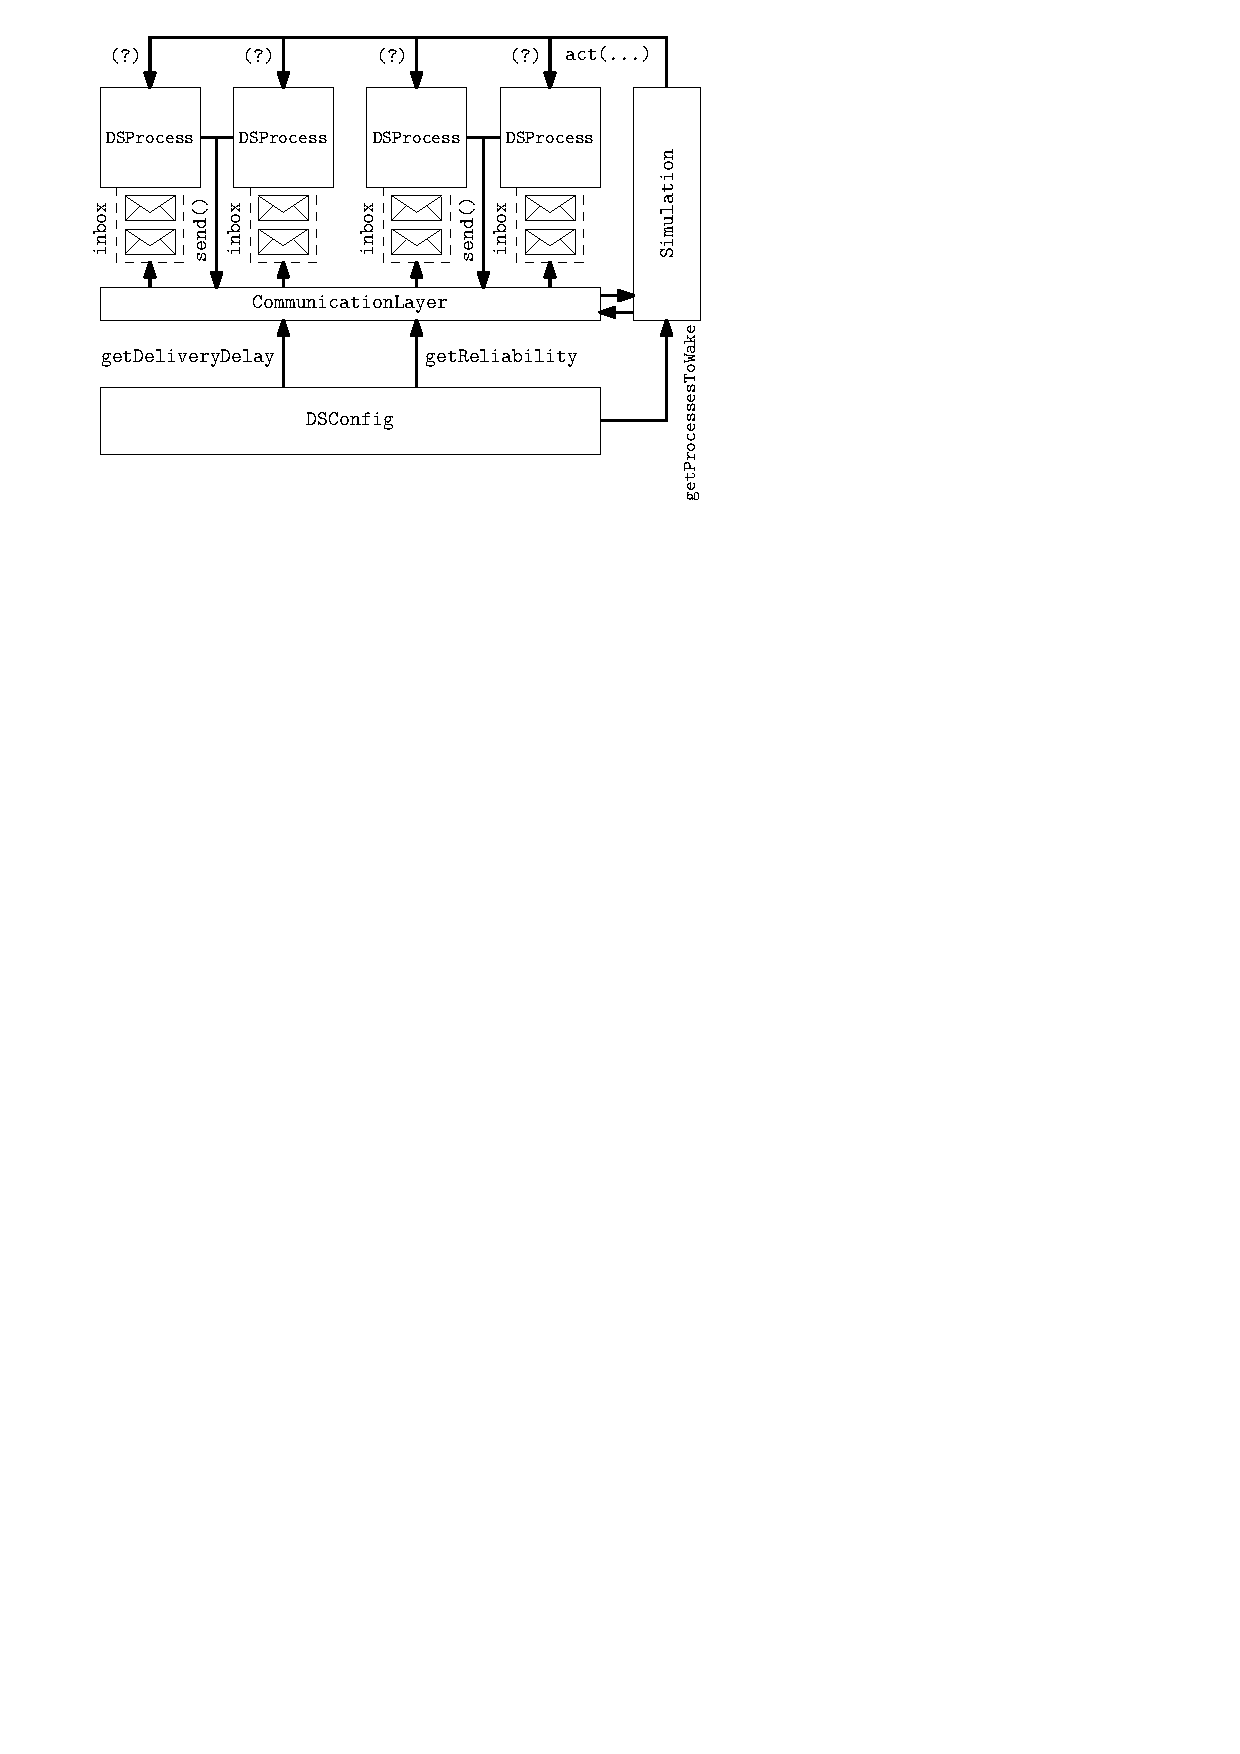
\includegraphics[width=0.8\linewidth]{10/figs/dsand.pdf}
\end{frame}

{\setbeamertemplate{frame footer}{\see{\url{http://goo.gl/a6BEMb}}}
\begin{frame}[fragile]
\frametitle{Jakými všemi způsoby může být následující kód proveden?}

\begin{minted}{c}
// CONFIG:
	getProcessesToWake() { return {"1", "2", "3"}; }
// PROCESS:
	int time = 0;
	int nid = Integer.parseInt(id);
	public void act() {
		time++;
		if(nid == time && nid != 3)
			send("3", new DummyMessage());
		while(!inbox.isEmpty()){
			Message m = inbox.poll();
			System.out.println(m.sender);
		}
	}
\end{minted}
% V idealnim pripade je resenim 1,2.
% Pokud se zpravy zpozduji, muze nastat take 2,1, a pokud se ztraceji tak 2 a take nemusi dojit k vypsani niceho.
% FIFO v zadani ne nutne znamena ze kumunikacni vrstva v simulaci je FIFO: FIFO muze byt kanal spojujici dva procesy.  V tom pripade je 2,1 spravne reseni pri zpozdovani zprav.
\end{frame}
}

\section{Detekce selhání v DS}

\begin{frame}
  \begin{minipage}{0.65\linewidth}
  
\includegraphics[width=.95\linewidth]{10/figs/hydra.png}
  \end{minipage}
  \pause
  \begin{minipage}{0.33\linewidth}
    {\Large \bf Vzpomeňte si na BFS}

    \vspace{1.2em}\hrule\vspace{1.2em}

    Co když spící/mrtvá hlava leží na nejkratší cestě?
  \end{minipage}
\end{frame}

\begin{frame}
  \frametitle{Detekce selhání}

  {\LARGE Když nám ,,umře`` důležitý proces, musíme být schopní se se situací vypořádat.}
  \hfill (Jinak nám celý DS zhavaruje)

  \pause\vspace{2.5em}

  \hfill \Large \faWarning \hspace{5pt} \bf Ale to musíme nejdřív zjistit, že ,,umřel``!

  \pause\hspace{2.5em}\hrule\vspace{1.5em}
  \begin{center}
    \LARGE \bf Jak na to?
  \end{center}
\end{frame}

{\setbeamertemplate{frame footer}{\see{{\tt DetectorProcess.java}\sep{\tt Run MainFD.java} v balíčku {\tt failure\_detector}}}
\begin{frame}
  \frametitle{Algoritmy na principu \emph{heart-beats}}

  \begin{itemize}
    \item Hearbeats jsou odesílány periodicky (každých $T$ ,,vteřin``)
    \item Nedostane-li proces heartbeat od procesu $p_j$ po dobu $T+\tau$ ,,vteřin``, považuje $p_j$ za mrtvý
  \end{itemize}

  \pause
  \begin{itemize}
    \item {\bf Centralizovaný heartbeat}
    \item {\bf Kruhový heartbeat}
    \item {\bf Všichni-všem (all-to-all) heartbeating}
  \end{itemize}

  \pause\vspace{1em}\hrule\vspace{1em}

  \begin{block}{Doprogramujte detekování selhání procesu na základě (all-to-all) heartbeating}
    Doimplementujte logiku detekování selhání procesu na základě (all-to-all) heartbeating v \texttt{DetectorProcess.java}. Následně spusťte scénář \texttt{MainFD.java}, ve kterém máte zajištěno, že selže právě jeden proces.
  \end{block}

\end{frame}
}

\begin{frame}
  \frametitle{Vlastnosti detektorů}

  \begin{itemize}
    \pause\item {\bf Úplnost}: každé selhání je časem detekováno aspoň jedním funkčním procesem
    \pause\item {\bf Přesnost}: nedochází k označení funkčního procesu za havarovaný
    \pause\item {\bf Rychlost}: čas do okamžiku, kdy první proces detekuje selhání
    \pause\item {\bf Škálovatelnost}: ani při velkém počtu agentů nedojde k zahlcení systému
  \end{itemize}

  \pause
  All-to-all heartbeating:
  \begin{itemize}
    \item[\bf\textcolor{BrickRed}{:-(}] Přesnost
    \item[\bf\textcolor{BrickRed}{:-(}] Škálovatelnost
  \end{itemize}

\end{frame}

\section{Čas a uspořádání událostí v DS  (1. část)}

\begin{frame}
  \frametitle{Fyzické hodiny}

  % In centralized systems, where one or more processors share a common bus, time isn't much of a concern. The entire system shares the same understanding of time: right or wrong, it is consistent.

  {\LARGE V centralizovaném systému je čas konzistentní...} \\
  {\large (procesy typicky sdílí \underline{jediné} hodiny)}

  \vspace{1em}

  Sdílené hodiny můžeme snadno využít pro:
  \begin{itemize}
    \item Koordinaci \\
          {\small (,,výpočet zahájíme v 11:47:23``)}
    \item Uspořádání kroků výpočtu \\
          {\small (logování, uspořádání procesů při přístupu do kritické sekce atd.)}
    \item ... a jiné
  \end{itemize}

\end{frame}

\begin{frame}
  \frametitle{Fyzické hodiny}

  % In centralized systems, where one or more processors share a common bus, time isn't much of a concern. The entire system shares the same understanding of time: right or wrong, it is consistent.

  {\LARGE V distribuovaném systému máme problém...} \\
  {\large (každý proces má \underline{vlastní} hodiny)}

  \vspace{1em}

  Možné problémy které hodiny mohou mít:
  \begin{itemize}
    \pause
    \item "Clock skew" \\
          {\small (hodiny A: 16:24, hodiny B: 16:32)}
    \pause
    \item "Clock drift" \\
          {\small (Hodiny začnou ve stejný čas, např. 12:00, ale po jedné hodině jedny ukazují 12:59 a druhé 13:01)}
  \end{itemize}

  \pause
  \vspace{1em}
  \hrule
  \vspace{1em}
  \Large \faWarning \hspace{5pt} \bf Často ale nepotřebujeme znát přesný čas, stačí znát skutečnou souslednost událostí. 

\end{frame}

% \begin{frame}
%   \frametitle{Fyzické hodiny}

%   \begin{center}
%     \LARGE Jak jsme na tom s fyzickým časem v případě DS?
%   \end{center}
%   Uvažujte například, že si chcete domluvit čas telefonátu s kamarádem, který je na druhém konci světa...

%   \vspace{1em}\hrule\vspace{1em}

%   \pause
%   Každý z Vás má své vlastní hodinky...
%   \begin{itemize}
%   	\pause\item Hodinky mohou ukazovat rozdílný čas (\emph{clock skew}) \\
%   	            {\small (jiná časová zóna, zapomenutá změna letního/zimního času, aj.)}
%   	\pause\item Nastavení stejného času před kamarádovým odletem nás nezachrání \\
%   				{\small (hodinky kamaráda se mohou například opožďovat -- \emph{clock drift})}
%   \end{itemize}

% \end{frame}

% \begin{frame}
%   \begin{center}
%   	\LARGE Co s tím?
%   \end{center}
%   \vspace{1em}
%   \begin{itemize}
%   	\pause\item Pokusíme se čas zobrazovaný na hodinkách sladit (\emph{synchronizovat}) \\
%   	            {\small (např. pošleme kamarádovi každých 15 minut SMS zprávu s naším časem)} \\[0.4em]

%   	            \pause\hfill \textcolor{BrickRed}{To ale nebude moc přesné... :-(} \\[2.2em]

%   	\pause\item Termín hovoru si domluvíme ad-hoc \\
%   				{\small (,,zhruba v 11:47 ti napíšu, že už mám čas -- ty mi zavolej zpět``)} \\[0.4em]

%   	            \pause\hfill {\LARGE Kauzalita!}

%                 \hfill Přijetí SMS $\rightarrow$ Zahájení hovoru
%   \end{itemize}
% \end{frame}

\begin{frame}
  \frametitle{Kauzalita}

  \begin{center}
  	{\LARGE Vztah příčiny a následku je v DS klíčový!} \\
  	(například, odpověď na dotaz následuje až po položení dotazu)

  	\vspace{1.5em}

  	\only<1>{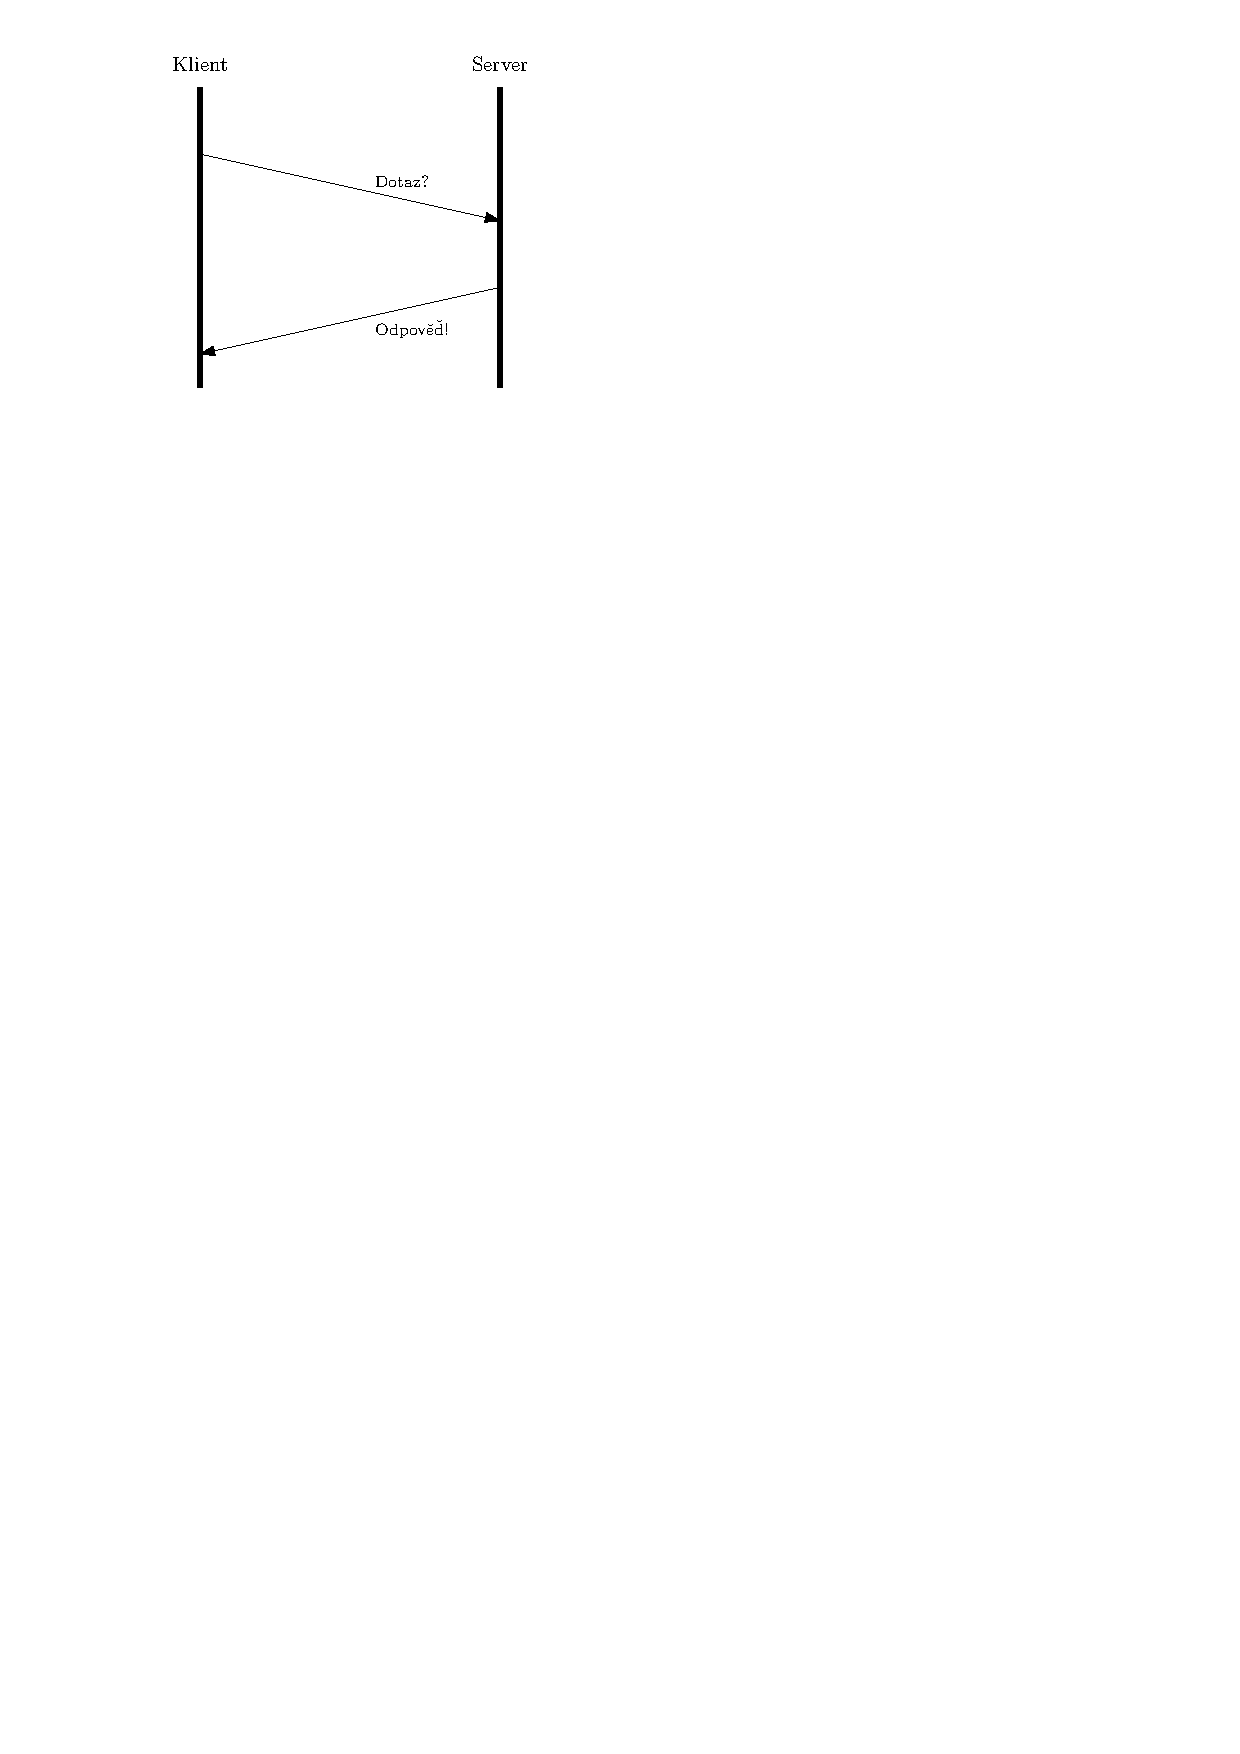
\includegraphics{10/figs/reqres.pdf}} %
  	\only<2>{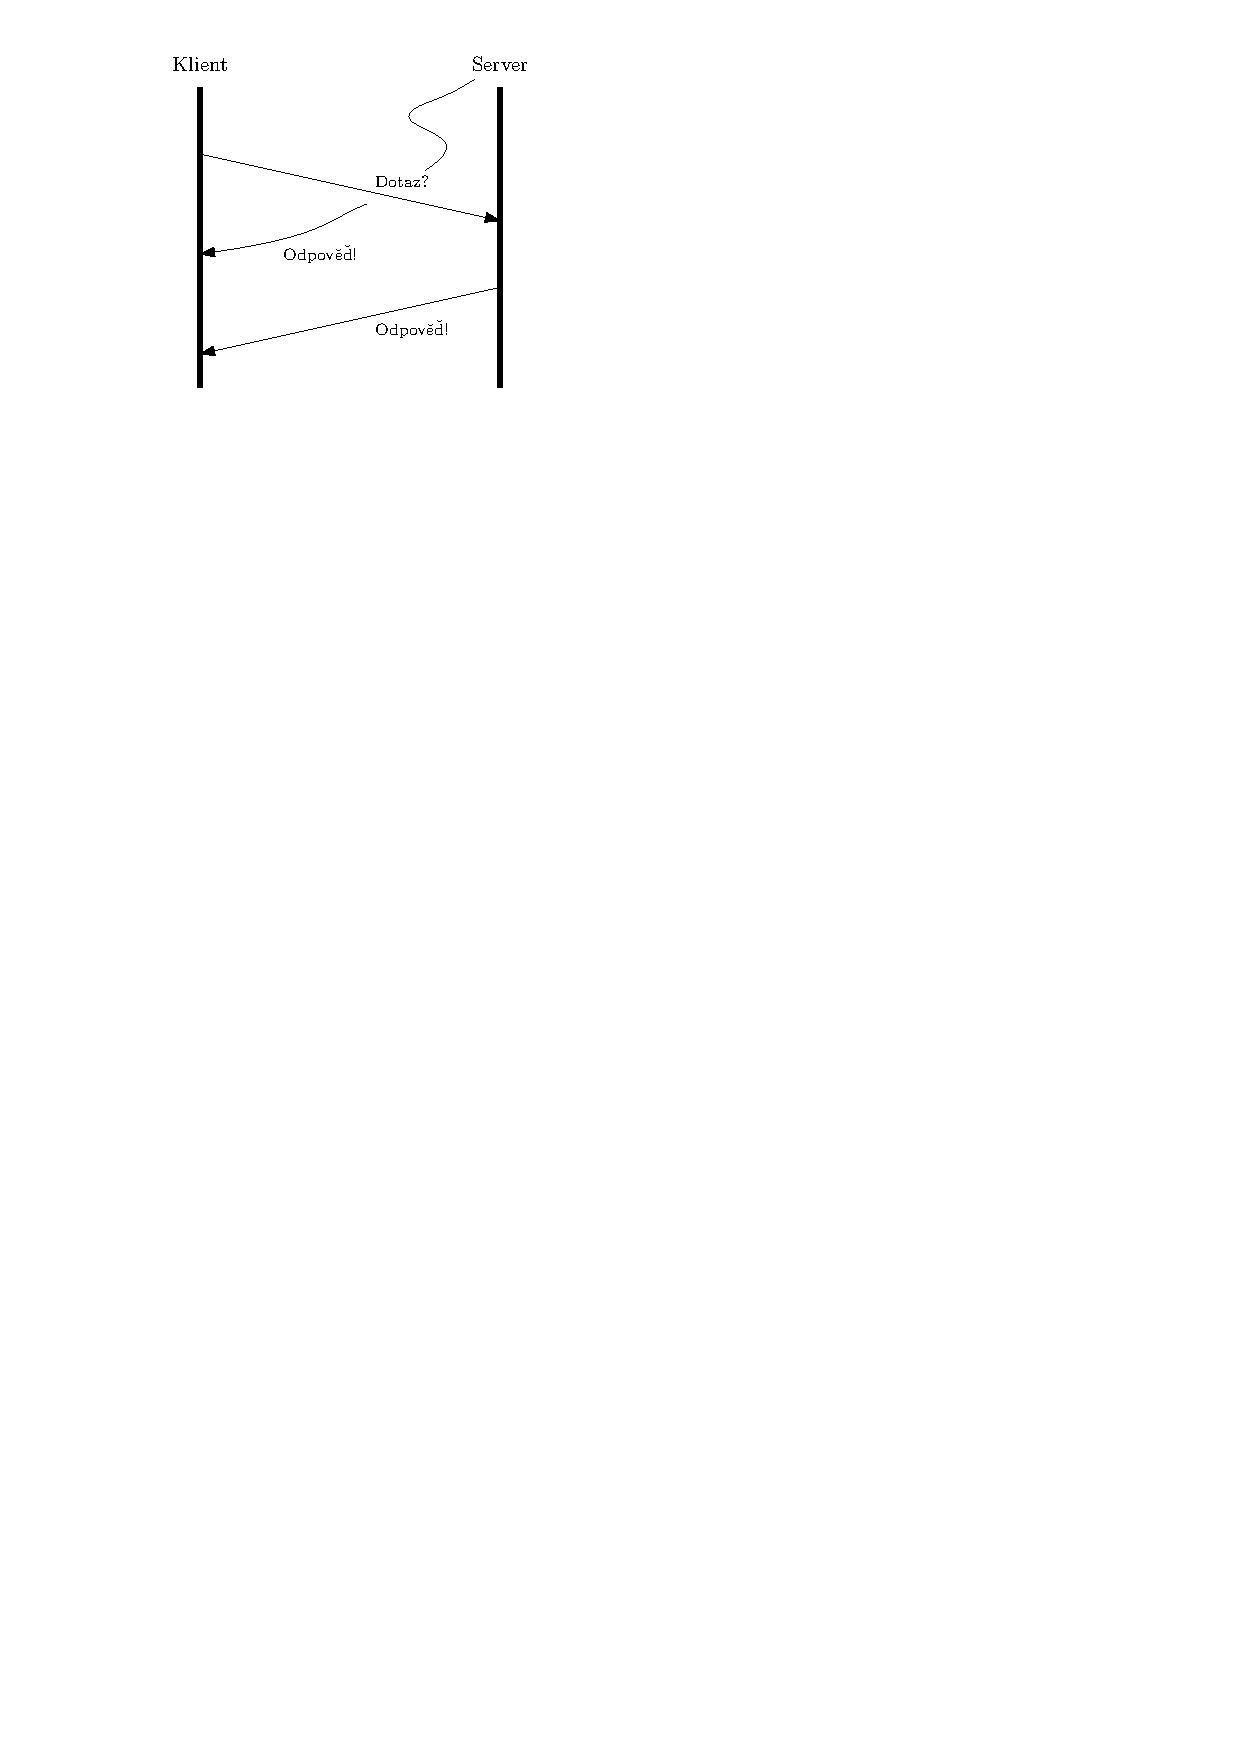
\includegraphics{10/figs/reqres2.pdf}} %
  	\only<3>{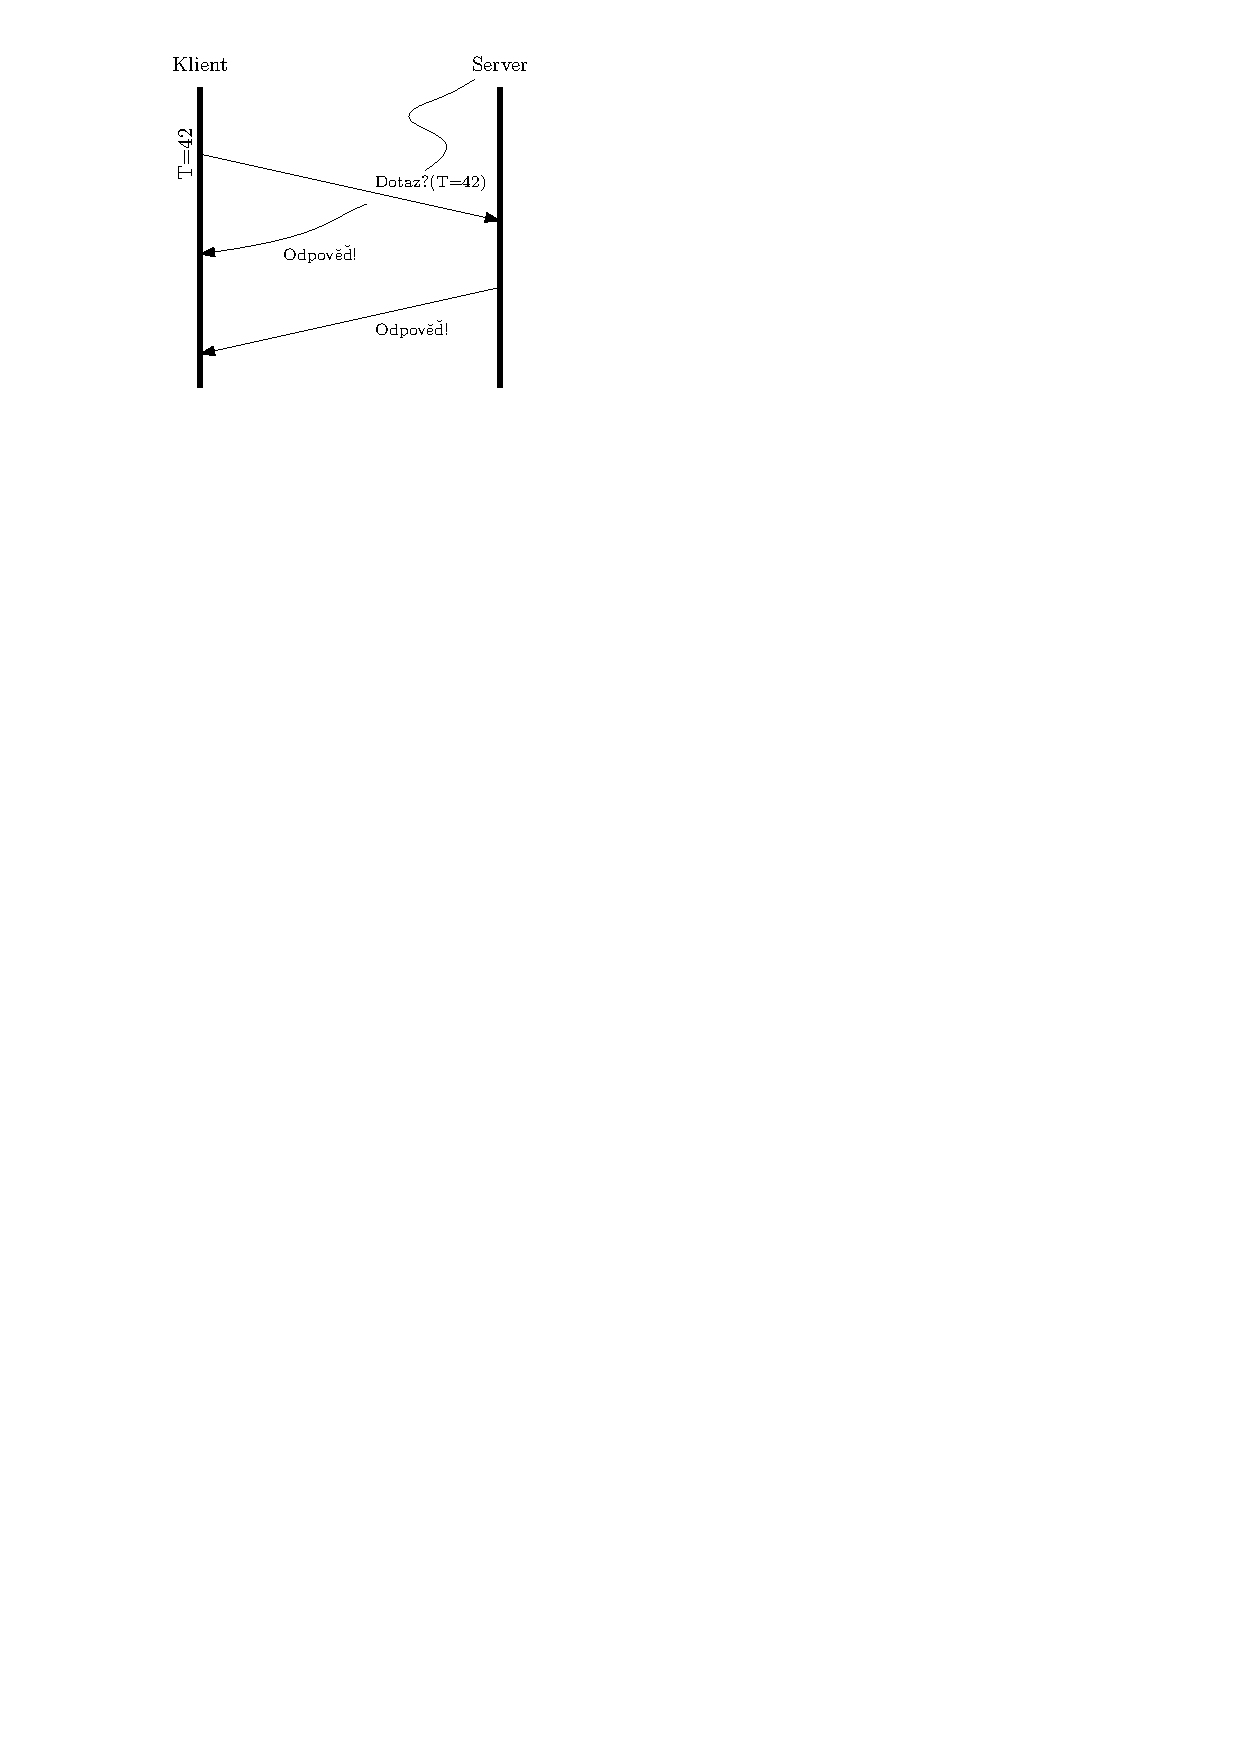
\includegraphics{10/figs/reqres3.pdf}} %
  	\only<4>{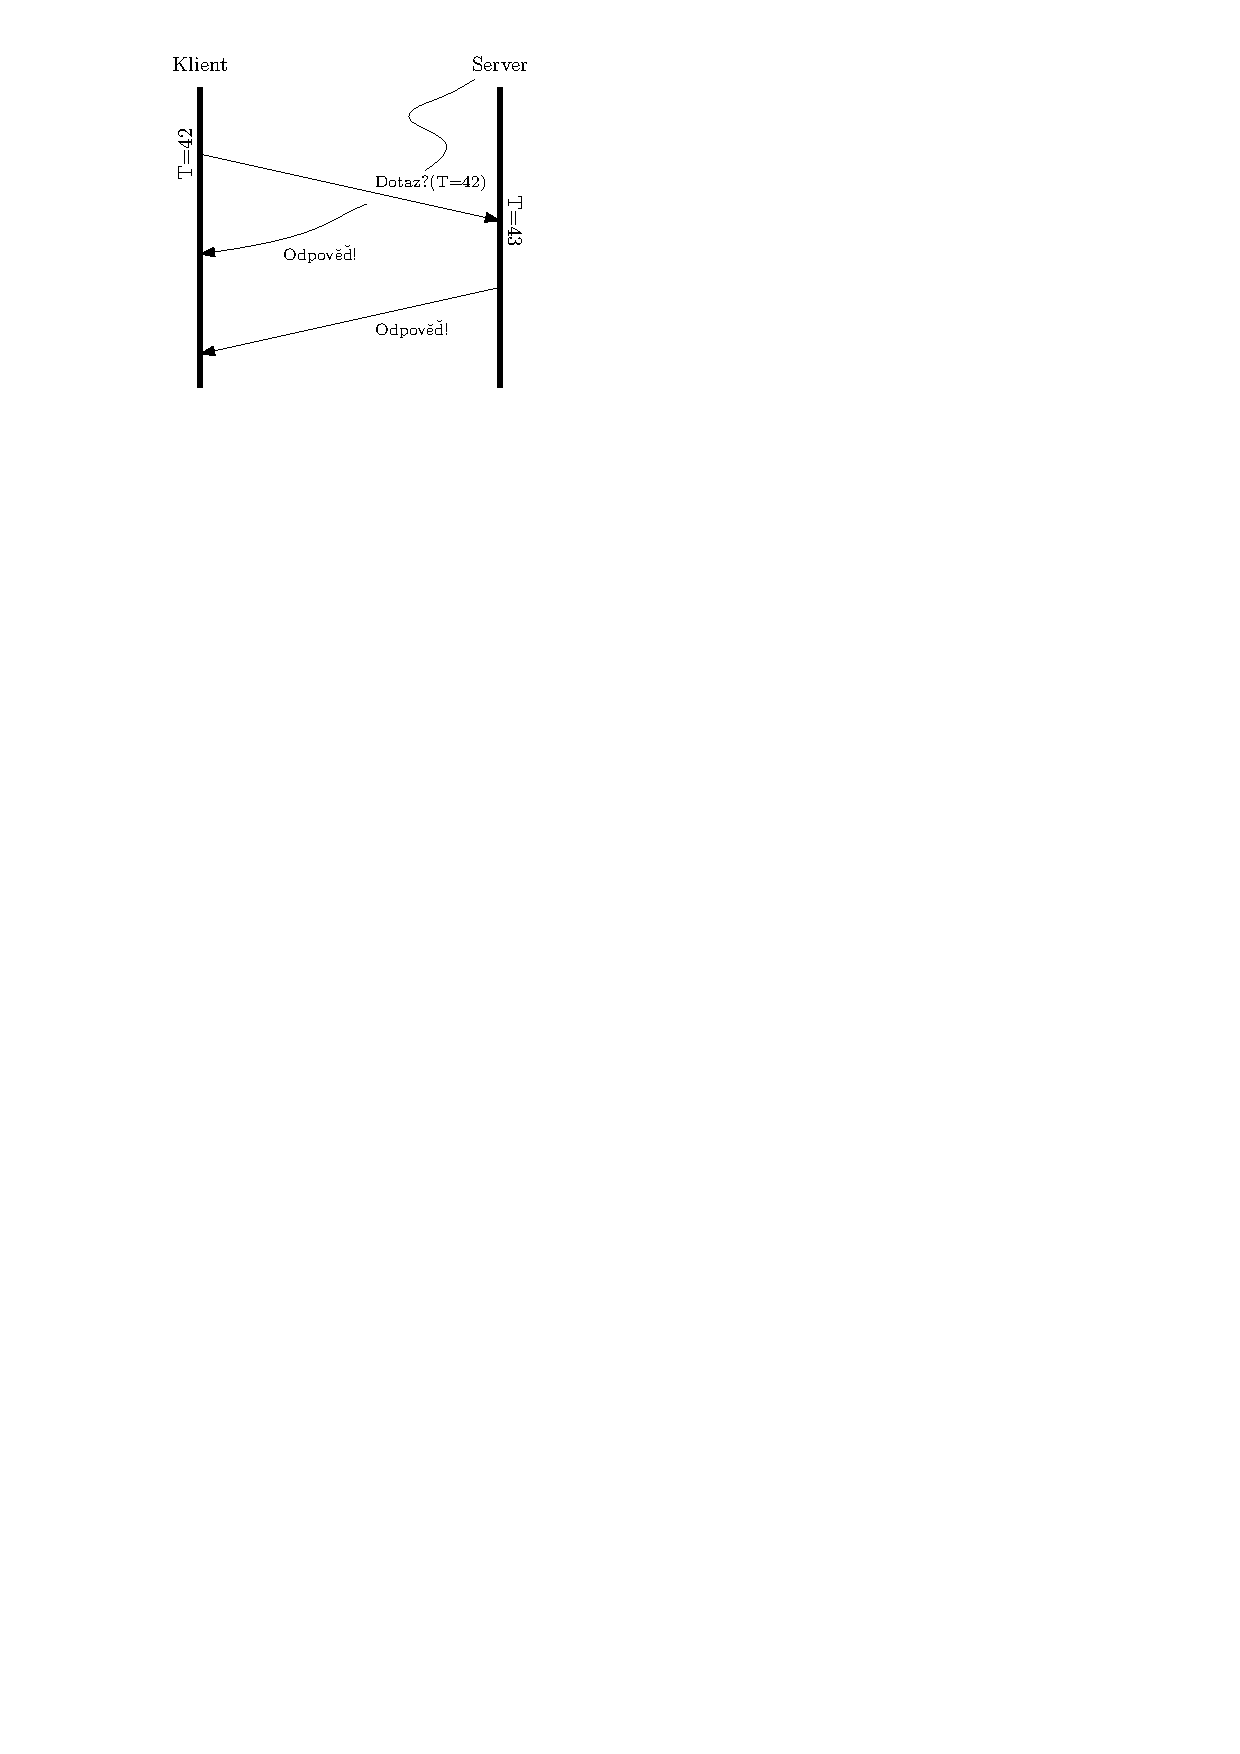
\includegraphics{10/figs/reqres4.pdf}} %
  	\only<5>{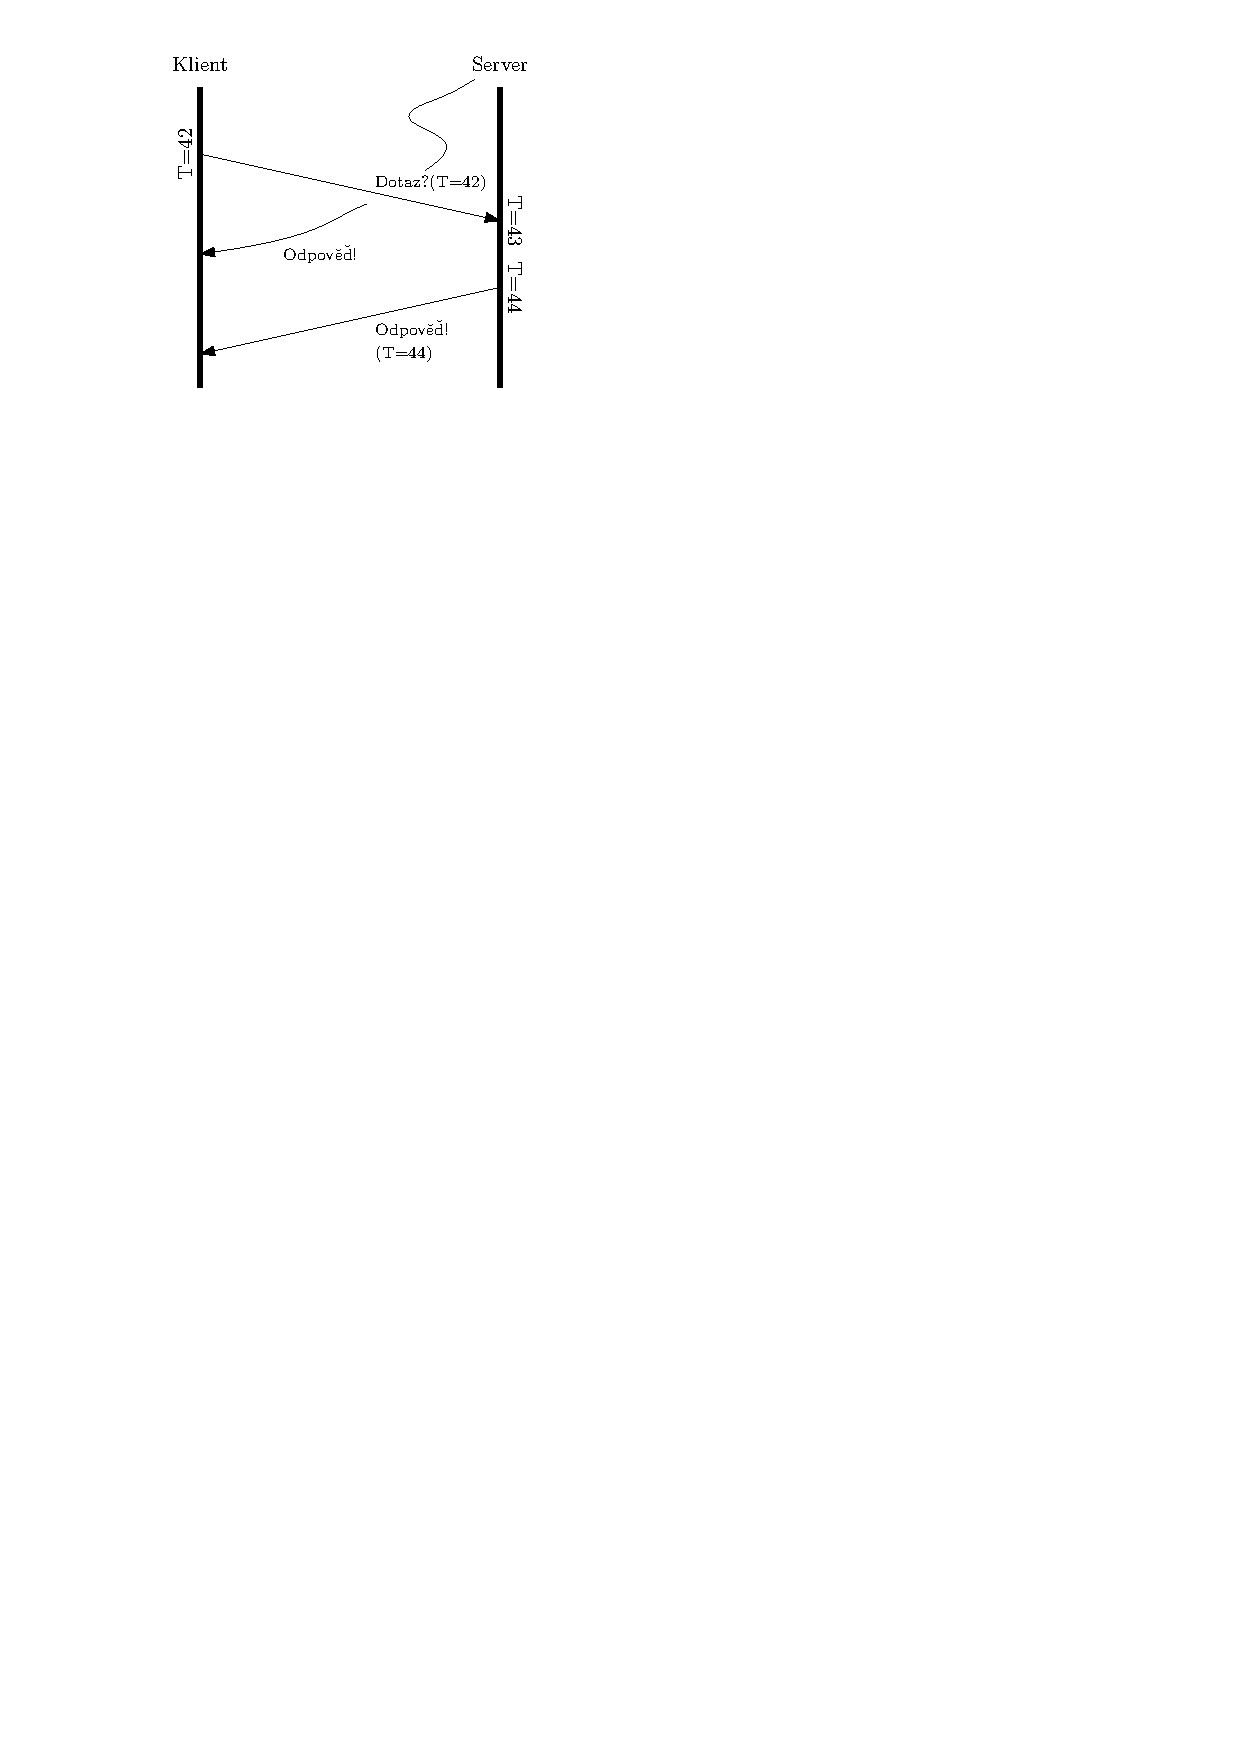
\includegraphics{10/figs/reqres5.pdf}} %
  	\only<6>{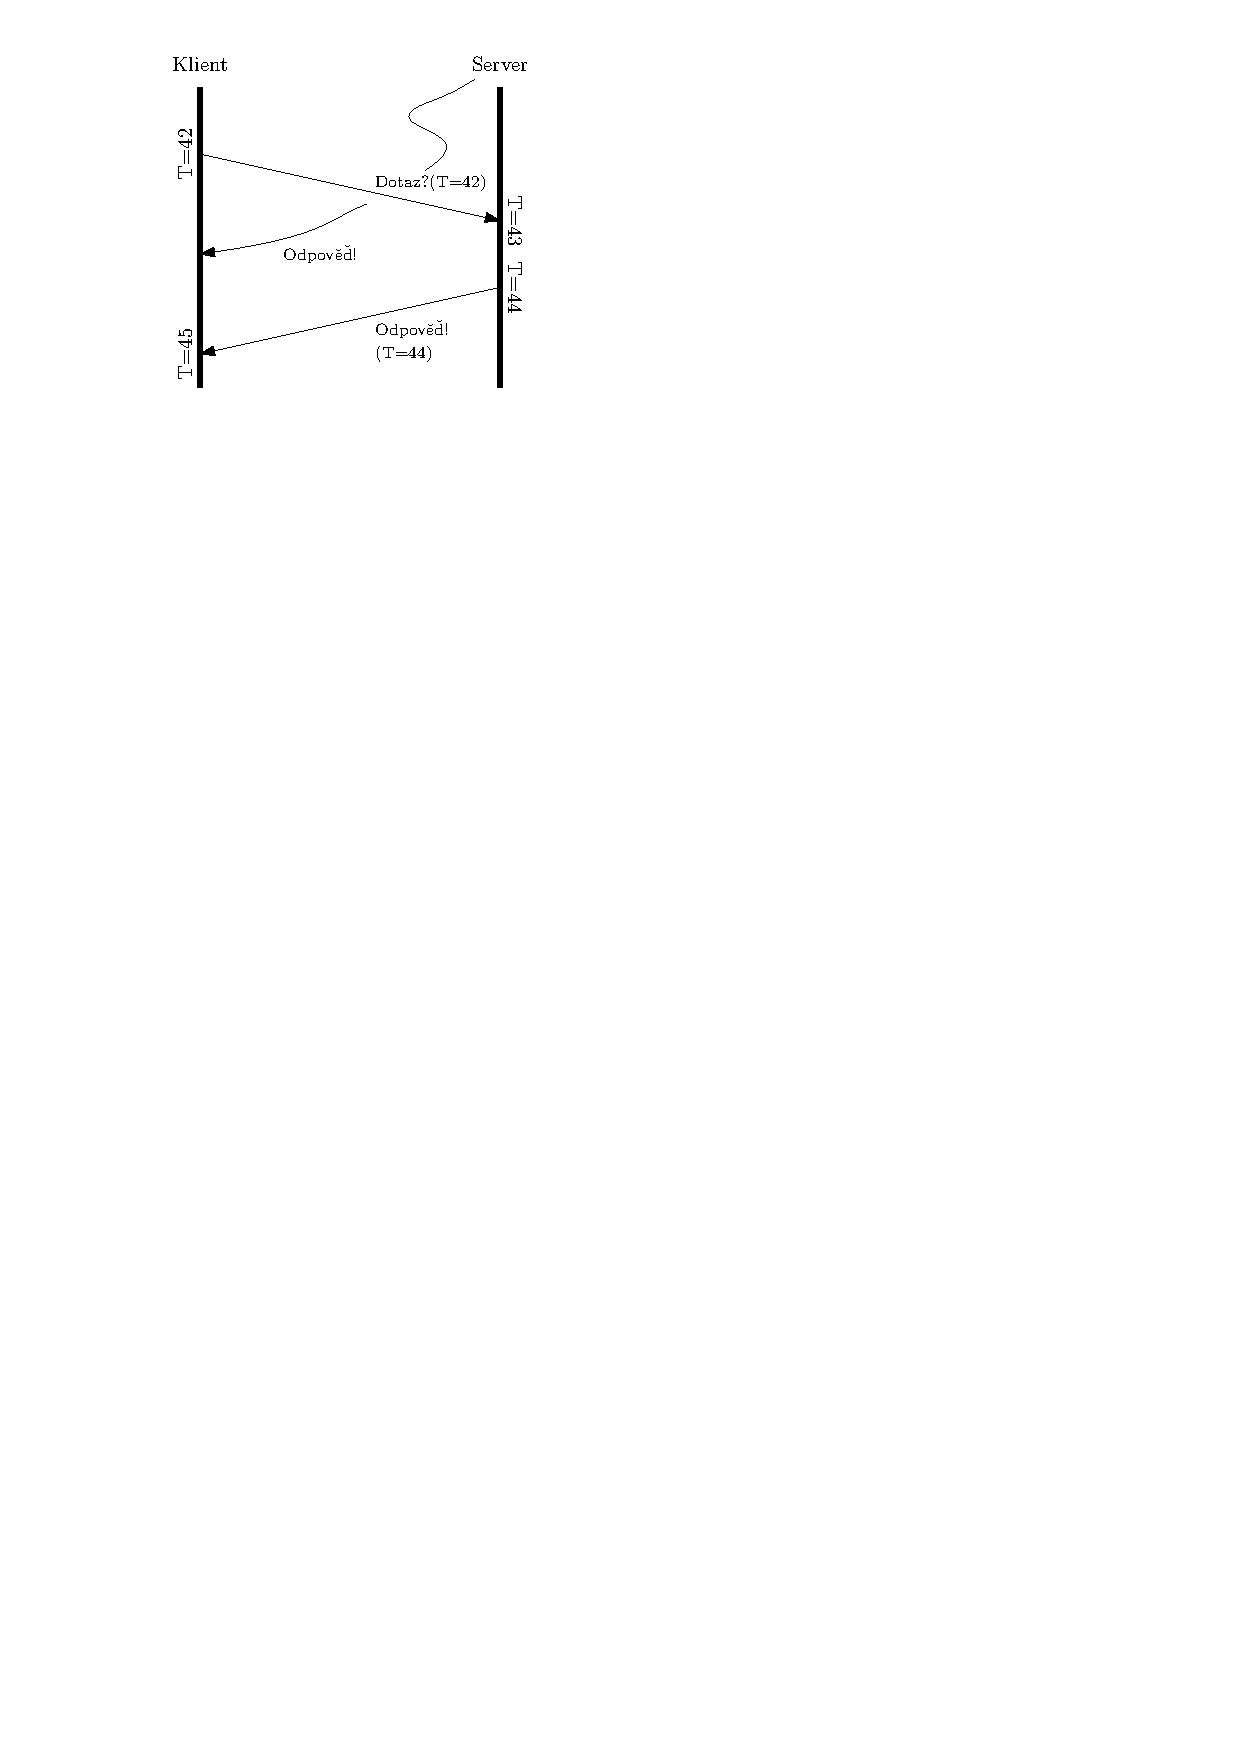
\includegraphics{10/figs/reqres6.pdf}} %
  	\only<7>{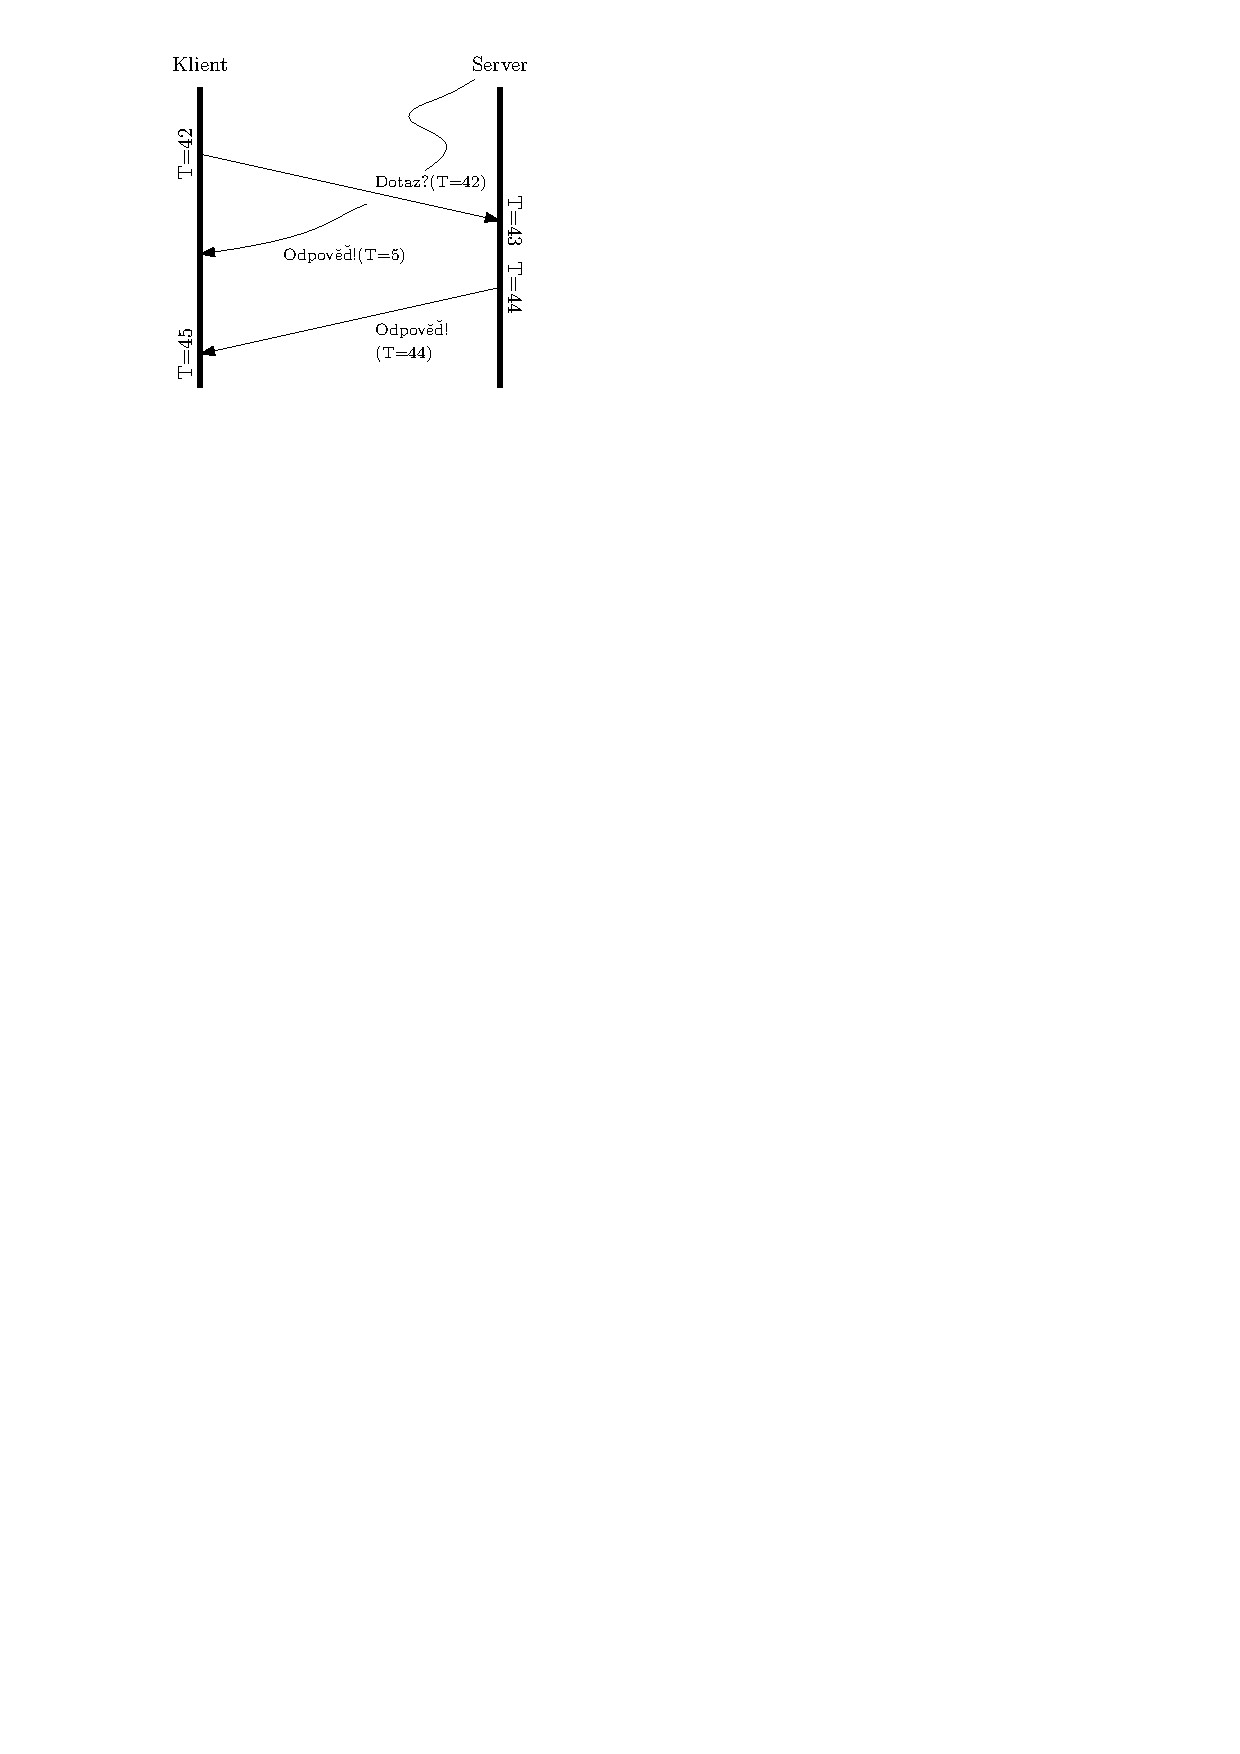
\includegraphics{10/figs/reqres7.pdf}} %
  \end{center}
\end{frame}

\begin{frame}
  \frametitle{Logický čas}

  \begin{center}
  	{\LARGE Právě jsme v našem DS zavedli logický čas! :-)} \\
  	(konkrétně Lamportovy skalární hodiny)
  \end{center}

  \pause\vspace{1em}\hrule\vspace{1em}

  Logický čas splňuje pouze kauzalitu!
  \begin{itemize}
  	\item Každé události $e$ přiřadíme časovou značku $T(e)$
  	\item Pokud je událost $e$ příčinou události $e'$, pak platí $T(e) < T(e')$ \\
		{\small (Ne nutně ale naopak!)}
  \end{itemize}
\end{frame}

\begin{frame}
  \frametitle{Skalární logické hodiny}

  \begin{center}
    \LARGE {\bf Lamportův algoritmus}
  \end{center}

  \vspace{1em}\hrule\vspace{1em}

  \begin{enumerate}
  	\pause\item Každý proces má svoje lokální logické hodiny \\
  	            \mintinline{java}{int logicalTime = 0}
  	\pause\item Před každou významnou událostí (obzvlášť posláním zprávy!) si proces lokální čas posune \\
  				\mintinline{java}{++logicalTime}
  	\pause\item Každé zprávě přiřadíme časovou značku $\texttt{msg.}T = \texttt{logicalTime}$ \\
  				{\small (Tím říkáme přijímajícímu procesu, ať si upraví svůj čas!)}
  	\pause\item Přijetí zprávy je následkem jejího odeslání -- pak musí platit $T(e) < T(e')$ \\
  				Po přijetí zprávy \texttt{msg} si proto musíme zaktualizovat svůj \texttt{logicalTime}:
  				\[ \texttt{logicalTime} = 1 + \max \lbrace \texttt{logicalTime},\ \texttt{msg.}T \rbrace \]
  \end{enumerate}

  %happens-before:
  %When comparing events on the same host, if event a occurs before event b then a happens-before b.
  %If one host receives a message sent by another host, the send happens-before the receive
  %If x occurs on P1 and y occurs on P2 and P1 and P2 have not exchanged messages then X and Y are said to be concurrent. If this is the case, we can't infer anything about the order of event x and event y. Please note, that this is only true if x and y don't exchange messages at all, even indirectly via third (or several) parties.
  %The relationship is transitive: if a happens before b, and b happens before c, then a happens before c.

  %We use this relationship to define our clock. Instead of a clock that keeps real time, it is basically a simple counter used to label events in a way that shows the happens-before relationship among them. Here are the rules that are used for updating the value of the logical clock on a host:
  %the counter is incremented before each event.
  %in the case of a send, the counter is incremented, and then the message is sent. The message should carry the new (incremented) timestamp.
  %in the case of a receive, the proper action depends on the value of the timestamp in the message. If the message has a higher timestamp than the receiver, the receiver's logical clock adopts the value sent with the message. In either case, the receiver's logical clock is incremented and the message is said to have been received at the new (incremented) clock value. This ensures that the messages is received after it was sent and after prior events on the receiving host.

  \vspace{1em}\hrule\vspace{1em}

  \pause\faWarning \hspace{3pt}
    \textbf{Skalární hodiny jsou stavebním kamenem mnoha algoritmů v DS!}
\end{frame}

% \begin{frame}
% \frametitle{Příklad: Lamportův logický čas}
% \begin{center}
% 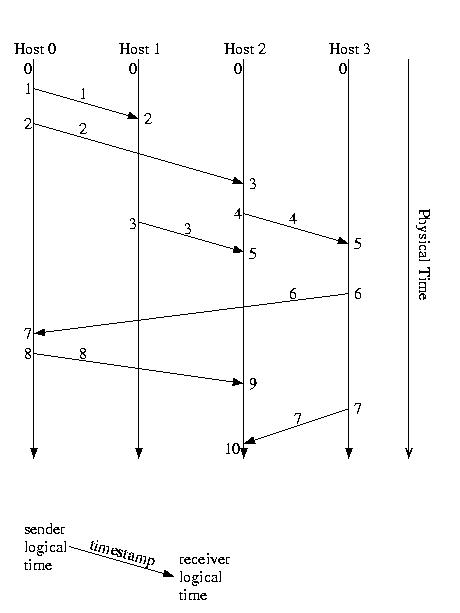
\includegraphics[width=.55\linewidth]{10/figs/lamporttime.jpg}
% \end{center}
% \end{frame}

\begin{frame}[t]
\frametitle{PDV Cloud}
\vspace{2.5em}
\begin{center}
\only<1,6->{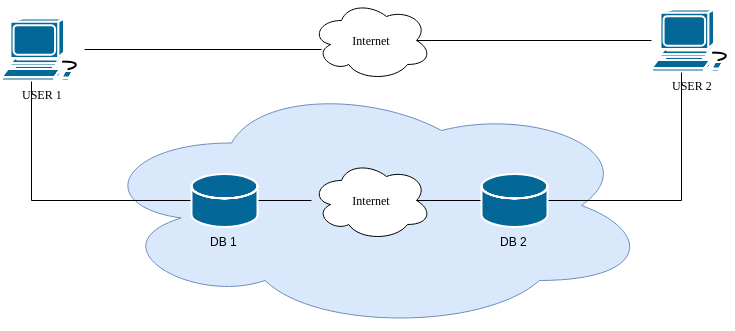
\includegraphics[scale=0.35]{10/figs/pdv_cloud.png}}%
\only<2>{\hspace{-6.4pt}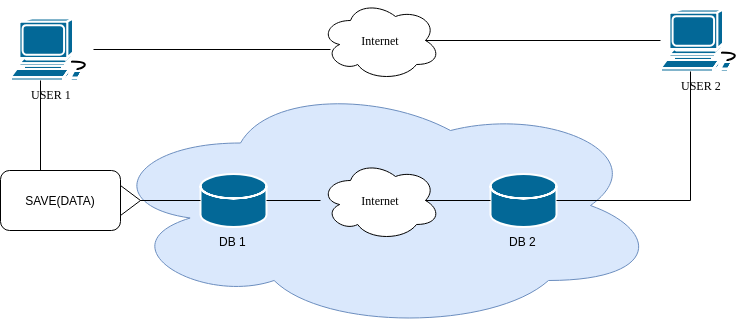
\includegraphics[scale=0.35]{10/figs/pdv_cloud_1.png}}%
\only<3>{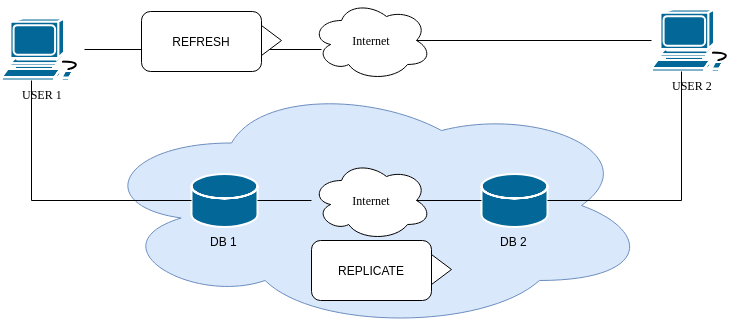
\includegraphics[scale=0.35]{10/figs/pdv_cloud_2.png}}%
\only<4>{\hspace{6.1pt}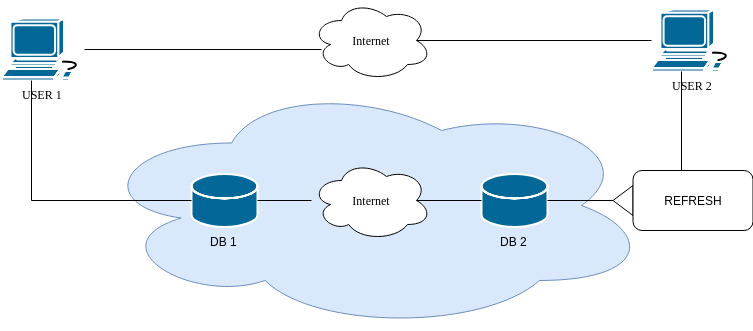
\includegraphics[scale=0.35]{10/figs/pdv_cloud_3.png}}%
\only<5>{\hspace{6.1pt}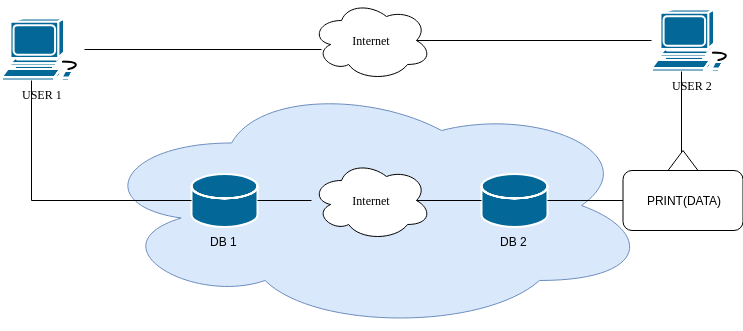
\includegraphics[scale=0.35]{10/figs/pdv_cloud_4.png}}%
\only<6>{\vspace{1em}\hrule\vspace{1em}
\Large K čemu bychom zde mohli chtít používat logické hodiny?}
% Zodpovězeno na dalších slidech [chceme detekovat, zda si User 2 refreshoval spravnou hodnotu.]
\end{center}
\end{frame}

{\setbeamertemplate{frame footer}{\see{{\tt ScalarClock.java} a {\tt ScalarTimestamp.java}\sep{\tt Run ScalarClockRun.java} v balíčku {\tt pdv\_cloud.scalar}}}
\begin{frame}

  \begin{block}{Doprogramujte Lamportovy logické hodiny}
    Doimplementujte logiku Lamportových logických hodin ve třídě \texttt{ScalarClock.java}. Následně spusťte scénář \texttt{ScalarClockRun.java}.
  \end{block}

  \pause\vspace{2em}
  \begin{center}
    \LARGE Co je v našem systému špatně?
  \end{center}

  \pause\faWarning \hspace{3pt}
    \textbf{Replikace může být pomalá. Druhý klient tak může číst stará data!}.

  \pause
  \vspace{2em}
  \begin{center}
    {\LARGE Jsme to schopní detekovat skalárními hodinami?}

    \hfill Doimplementujte metodu \texttt{isCausalityForProcessViolated}

    \hfill Pak zkuste spustit scénář \texttt{ScalarDSConfigBombarding}   % Bombarding rozbije právě naimplementovanou detekci tím způsobem, že bude navyšovat čas na databázi a tím pádem budeme detekovat porušení kauzality pokaždé, přestože k němu třeba vůbec nedošlo.
  \end{center}

\end{frame}
}

\begin{frame}
  \begin{center}
    \LARGE Jak protokol upravit, aby nedocházelo k porušení kauzality?
  \end{center}

  \pause\vspace{1em}\hrule\vspace{1em}
  Možností je mnoho, například:
  \begin{itemize}
    \pause\item Před odesláním \texttt{REFRESH} zprávy si počkat na potvrzení od databáze \\
                {\small (Odeslání \texttt{REFRESH} zprávy je kauzálním následkem úspěšné replikace)}
    \pause\item Pozdržet vyhodnocení dotazu do doby, než replikace proběhne \\
                {\small (Druhému uživateli můžeme poslat, že má požadovat data zapsaná nejdříve v daném logickém čase)}
  \end{itemize}
  %Very shortly, we'll talk about designing a communication mechanism that avoid causality violations.
  \pause
  \begin{itemize}
    \item[\faWarning] \bf Obecně chceme, aby události $e_1$, $e_2$, které mají proběhnout po sobě (tj. například čtení až po replikaci) byly ve vztahu kauzální závislosti.
  \end{itemize}
\end{frame}

% %2022-04-19 - presun Vektorovych hodin do dalsiho cviceni
% \begin{frame}[fragile]
%   Chceme provést následující dvě operace v daném pořadí:
%   \begin{enumerate}
%     \item Převést všechny peníze z účtu v bance A na účet v bance B (\texttt{transfer\_all(A, B)})
%     \item Převést všechny peníze z účtu v bance B na účet v bance C (\texttt{transfer\_all(B, C)})
%   \end{enumerate}

%   \begin{minted}{c}
%   	void transfer_all(int & from, int & to) {
%   		to += from;
%   		from = 0;
%   	}

%   	transfer_all(A, B);
%   	transfer_all(B, C);
%   \end{minted}
% \end{frame}

% \begin{frame}[t]
%   \frametitle{Jak to provést v distribuovaném systému?}
%   \begin{center}
%   	\only<1>{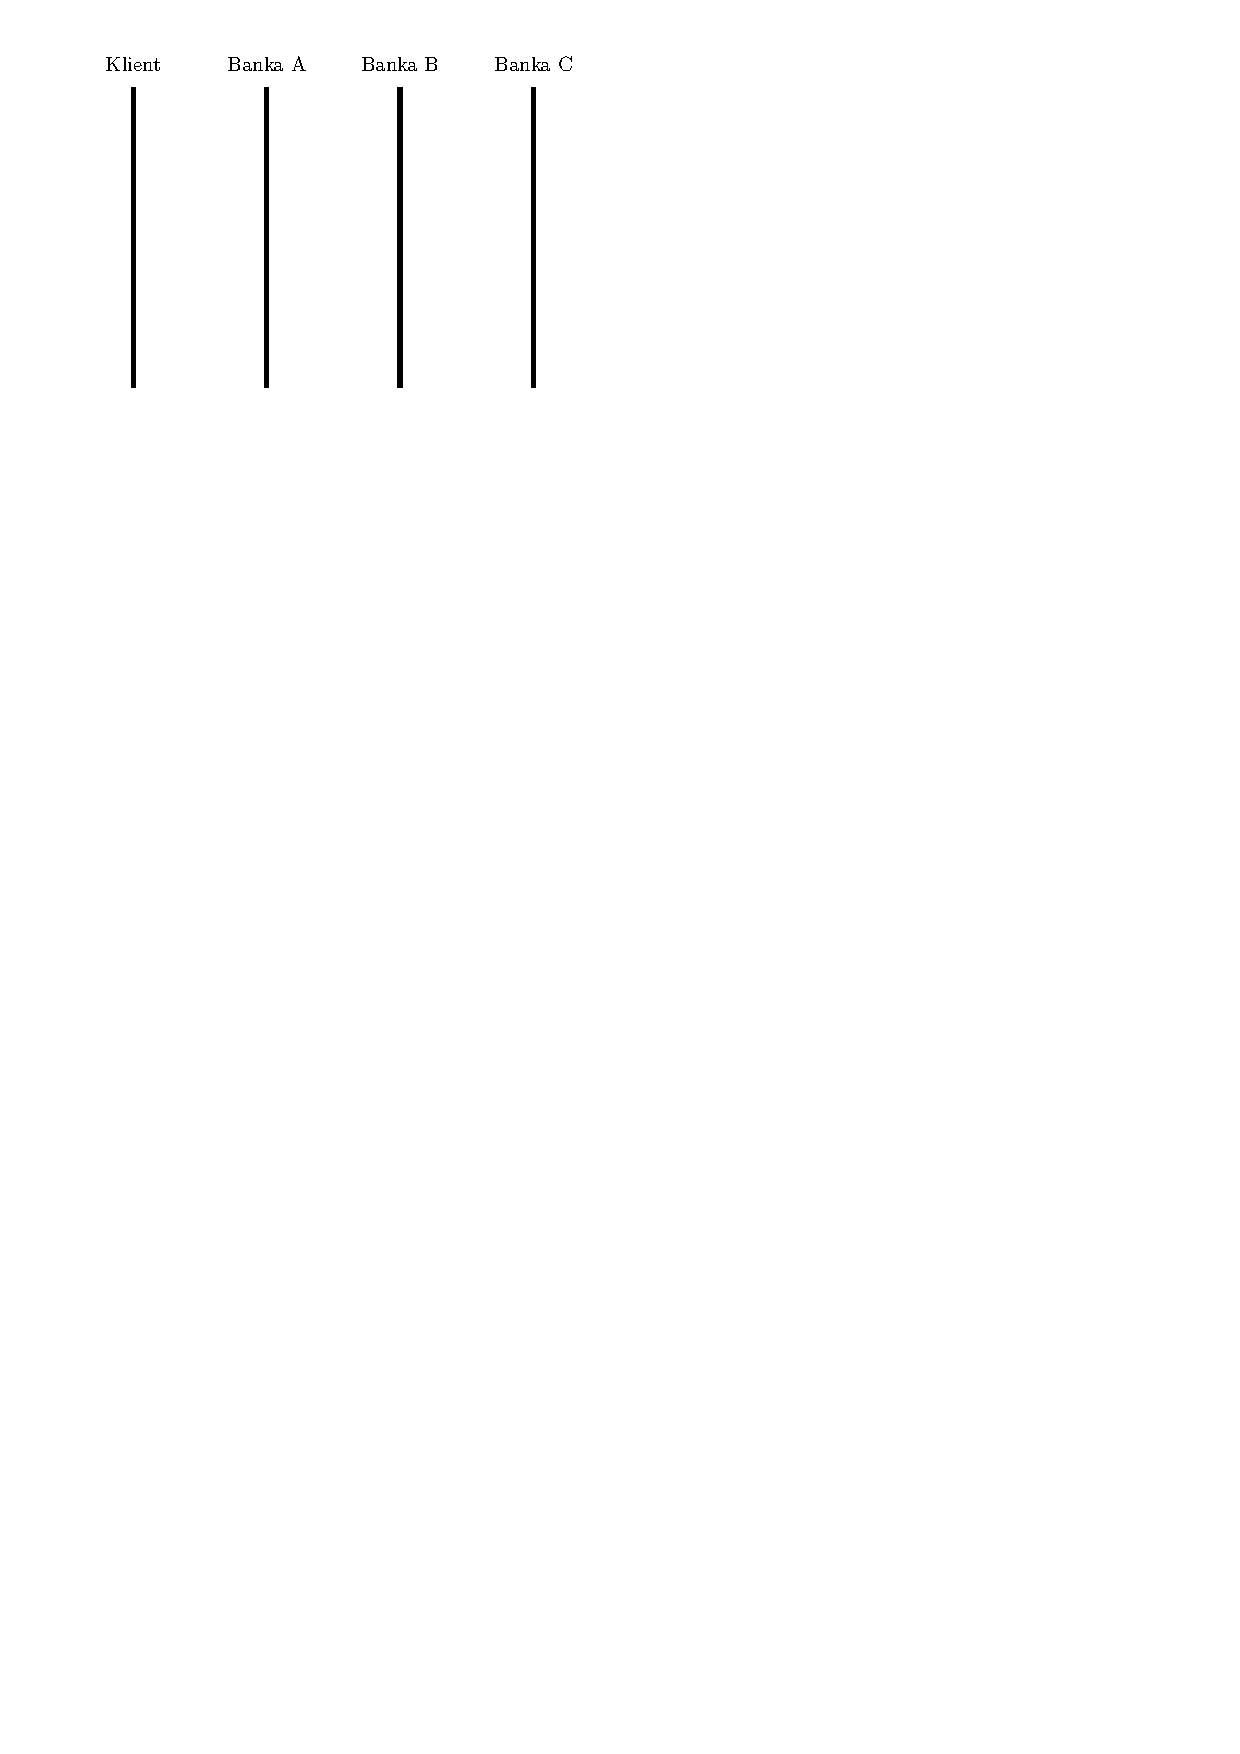
\includegraphics{10/figs/bank1.pdf}}%
%   	\only<2>{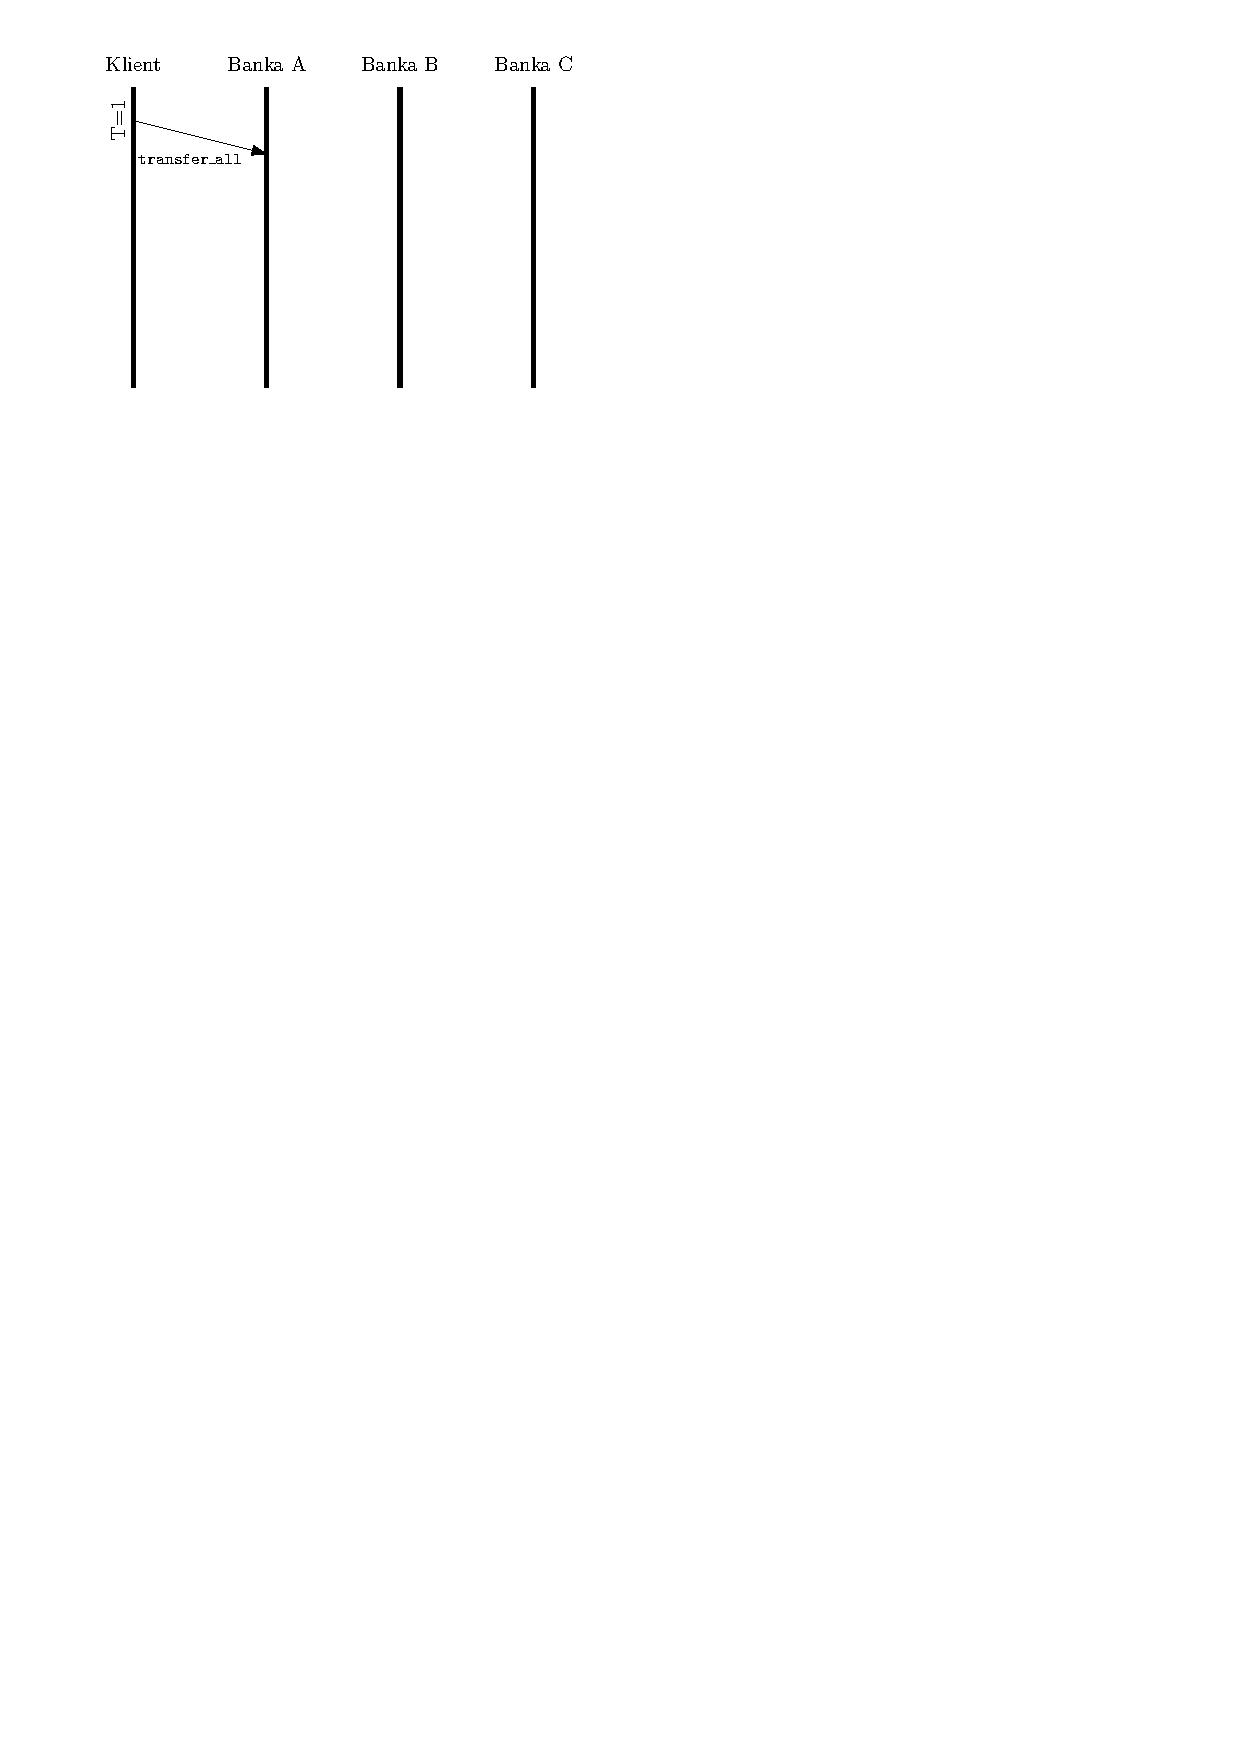
\includegraphics{10/figs/bank2.pdf}}%
%   	\only<3>{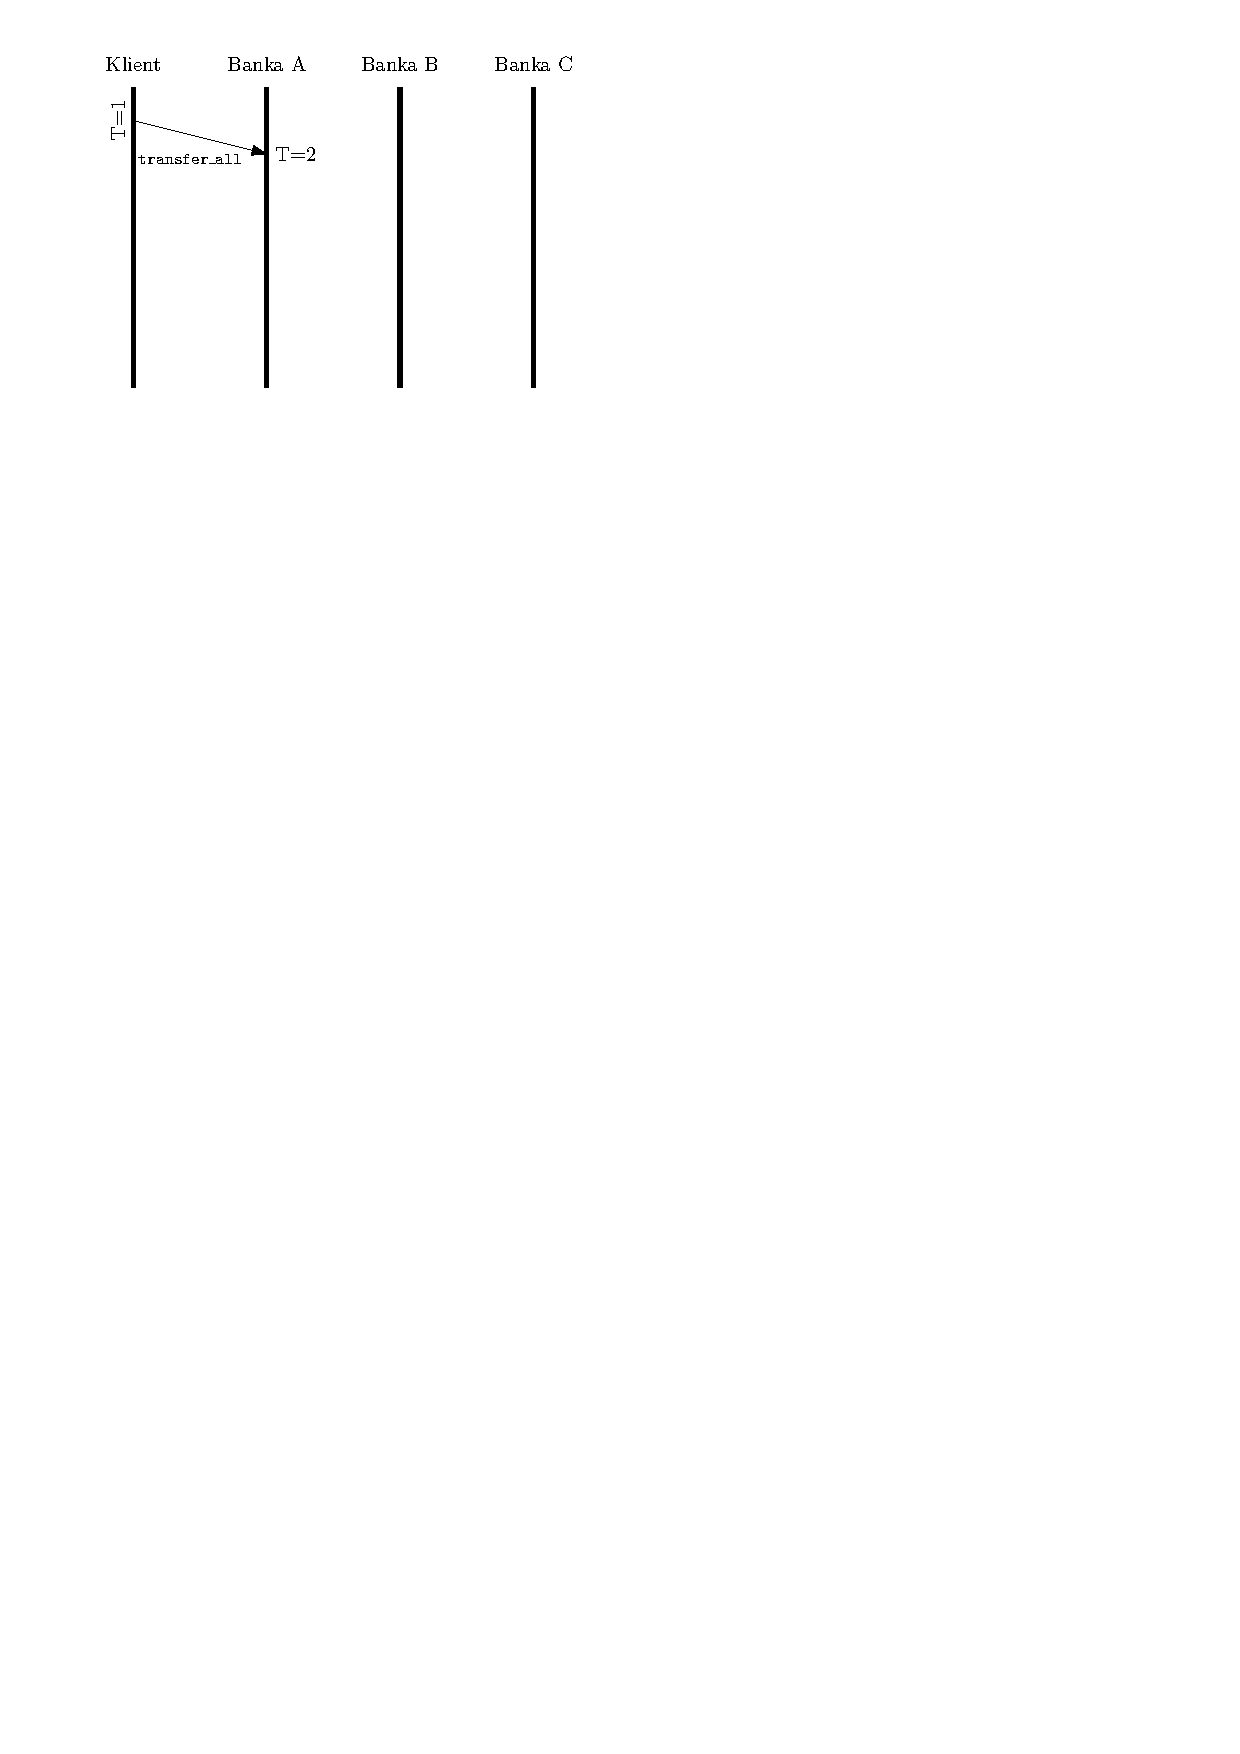
\includegraphics{10/figs/bank3.pdf}}%
%   	\only<4>{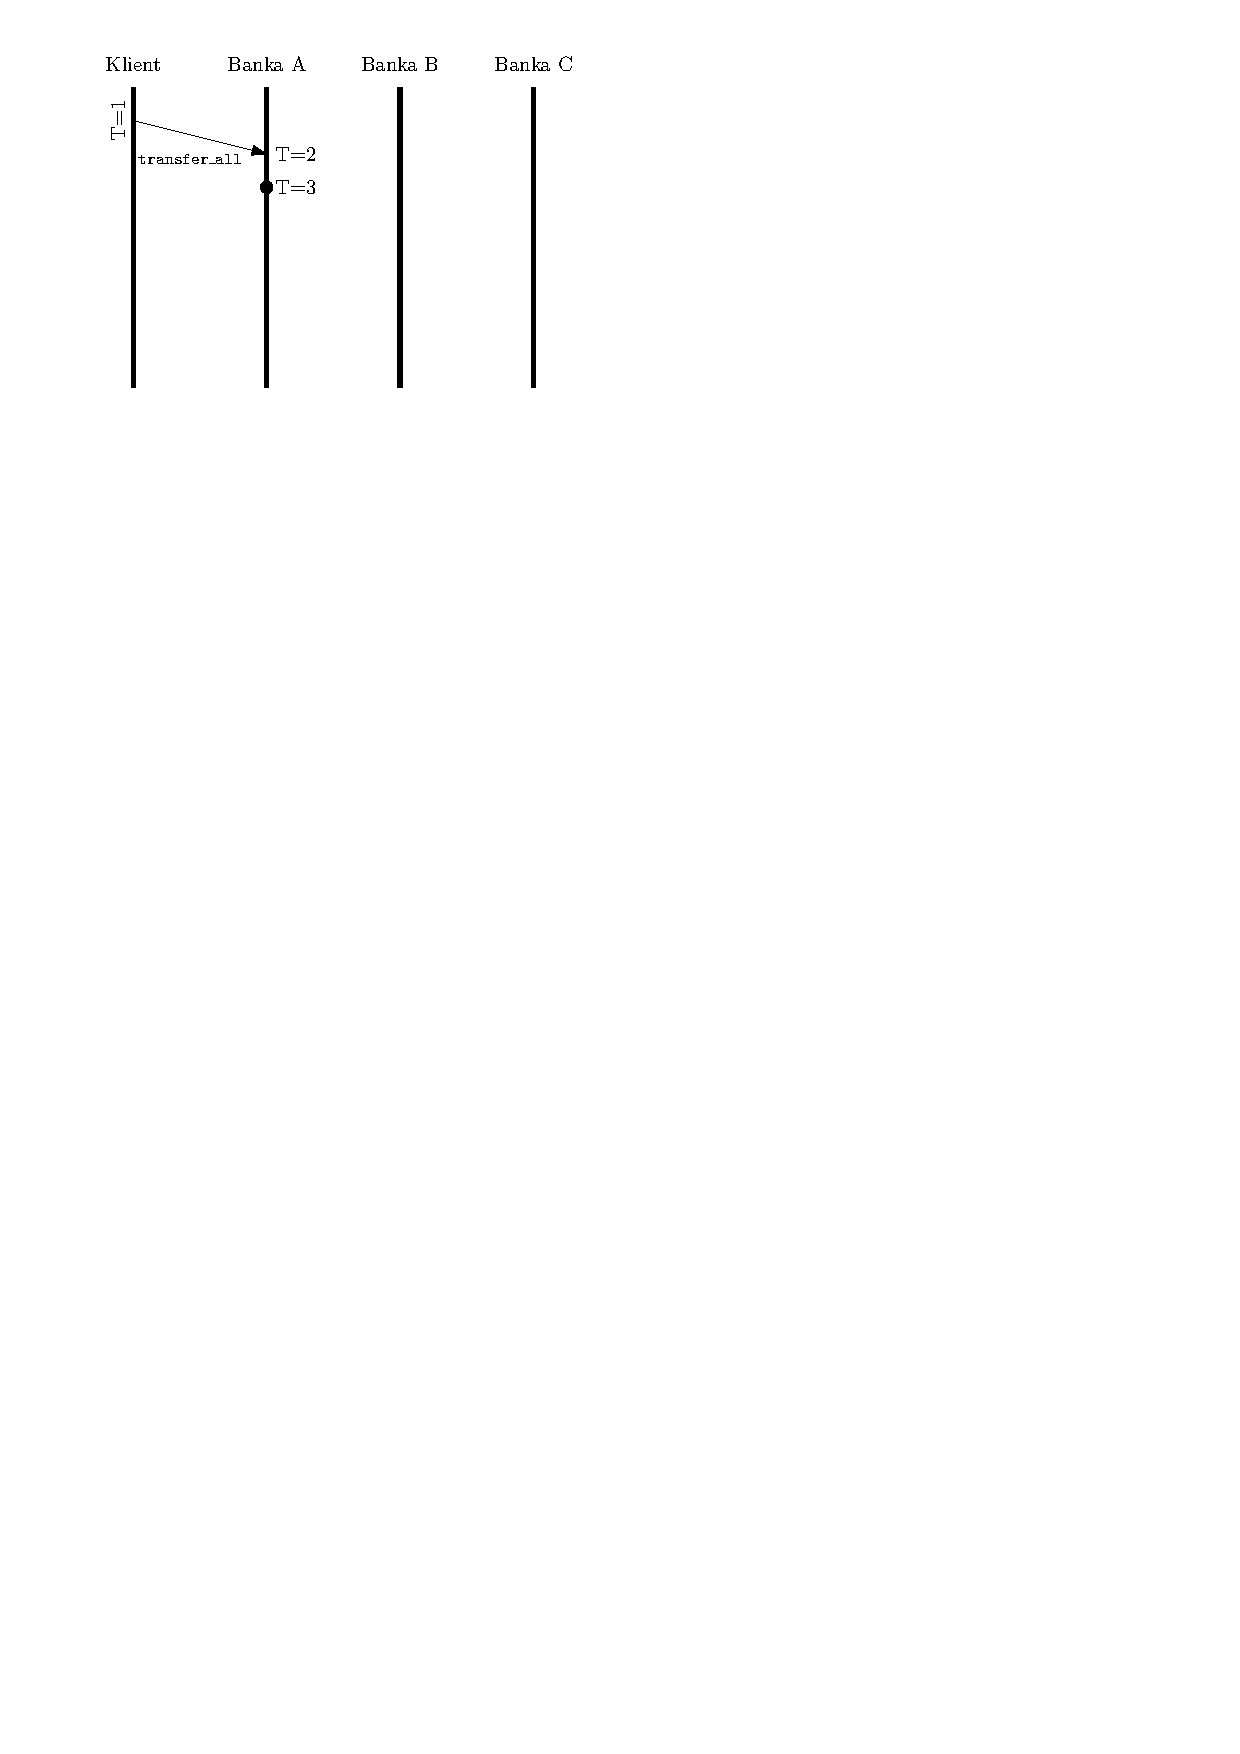
\includegraphics{10/figs/bank4.pdf}}%
%   	\only<5>{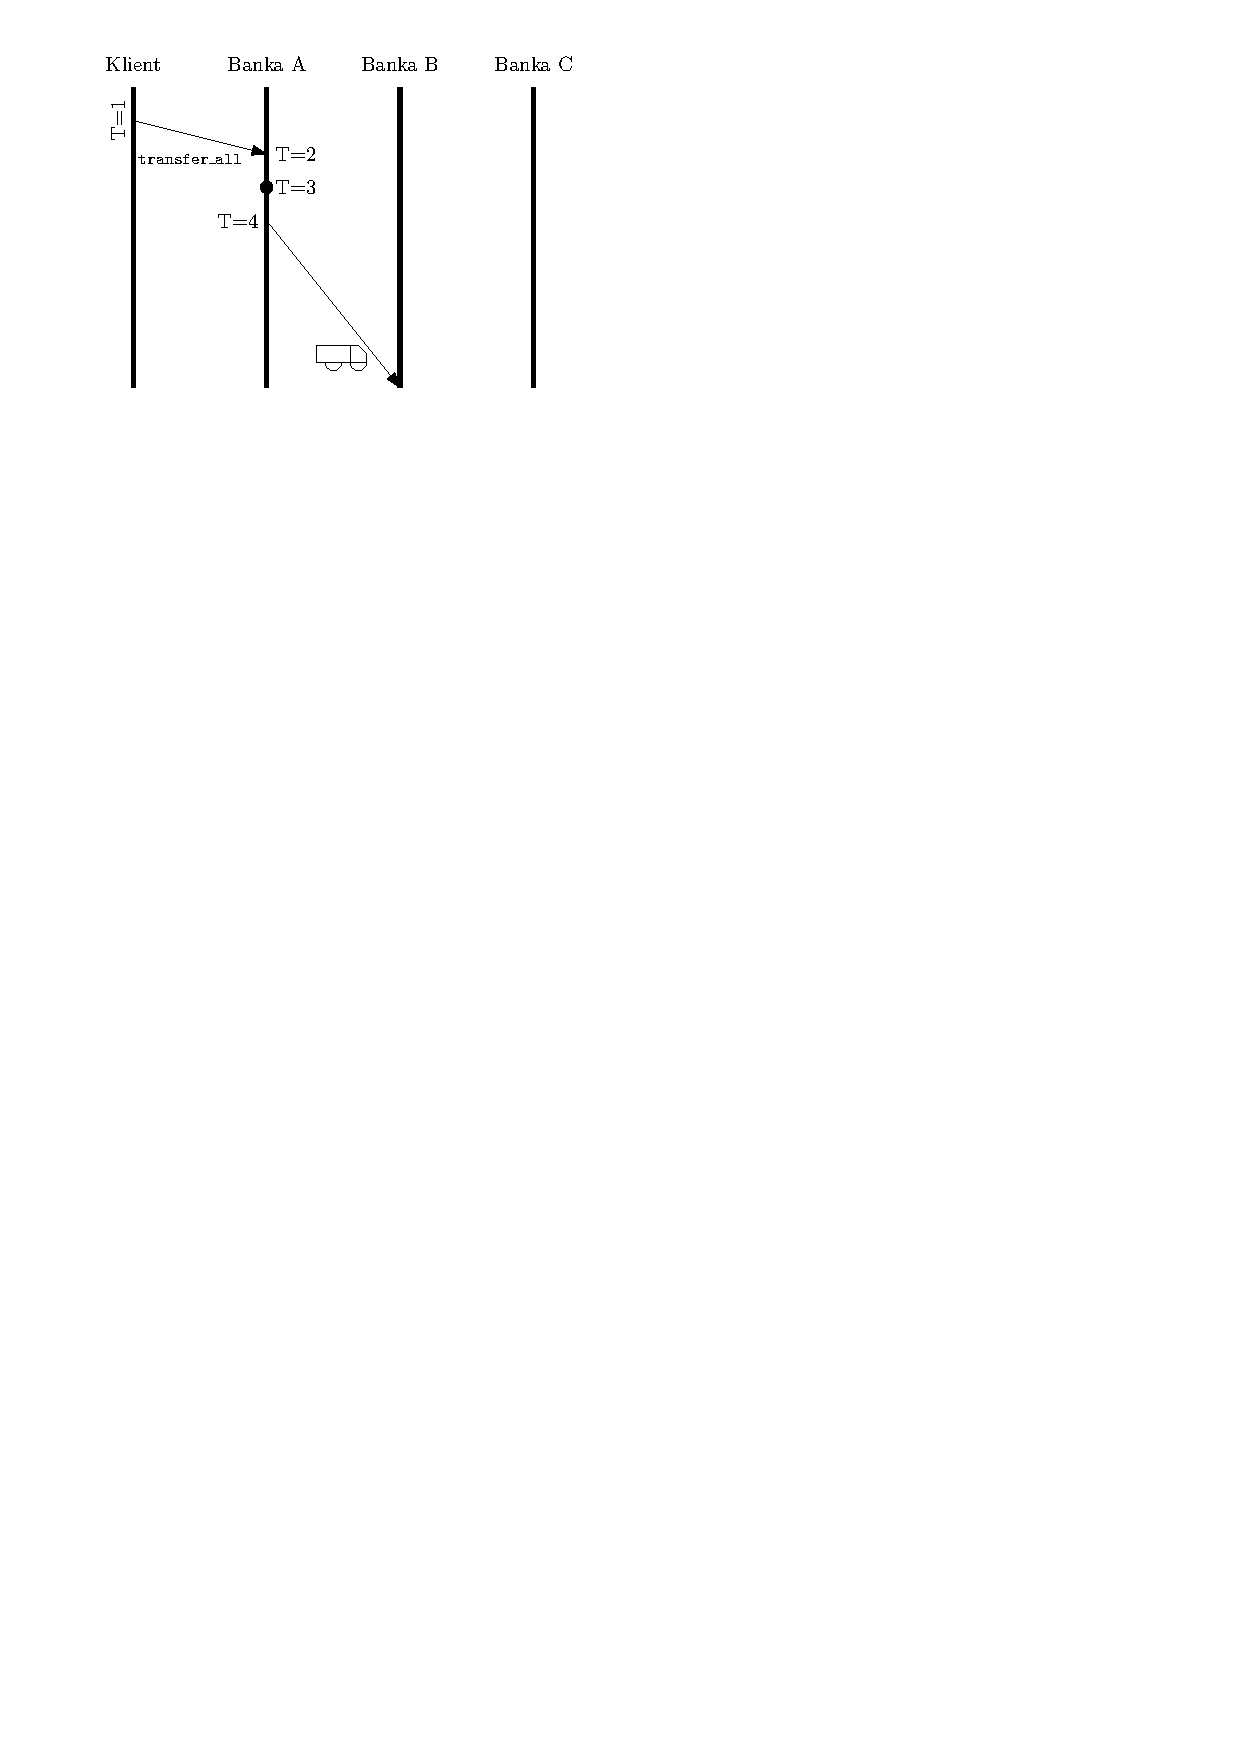
\includegraphics{10/figs/bank5.pdf}}%
%   	\only<6>{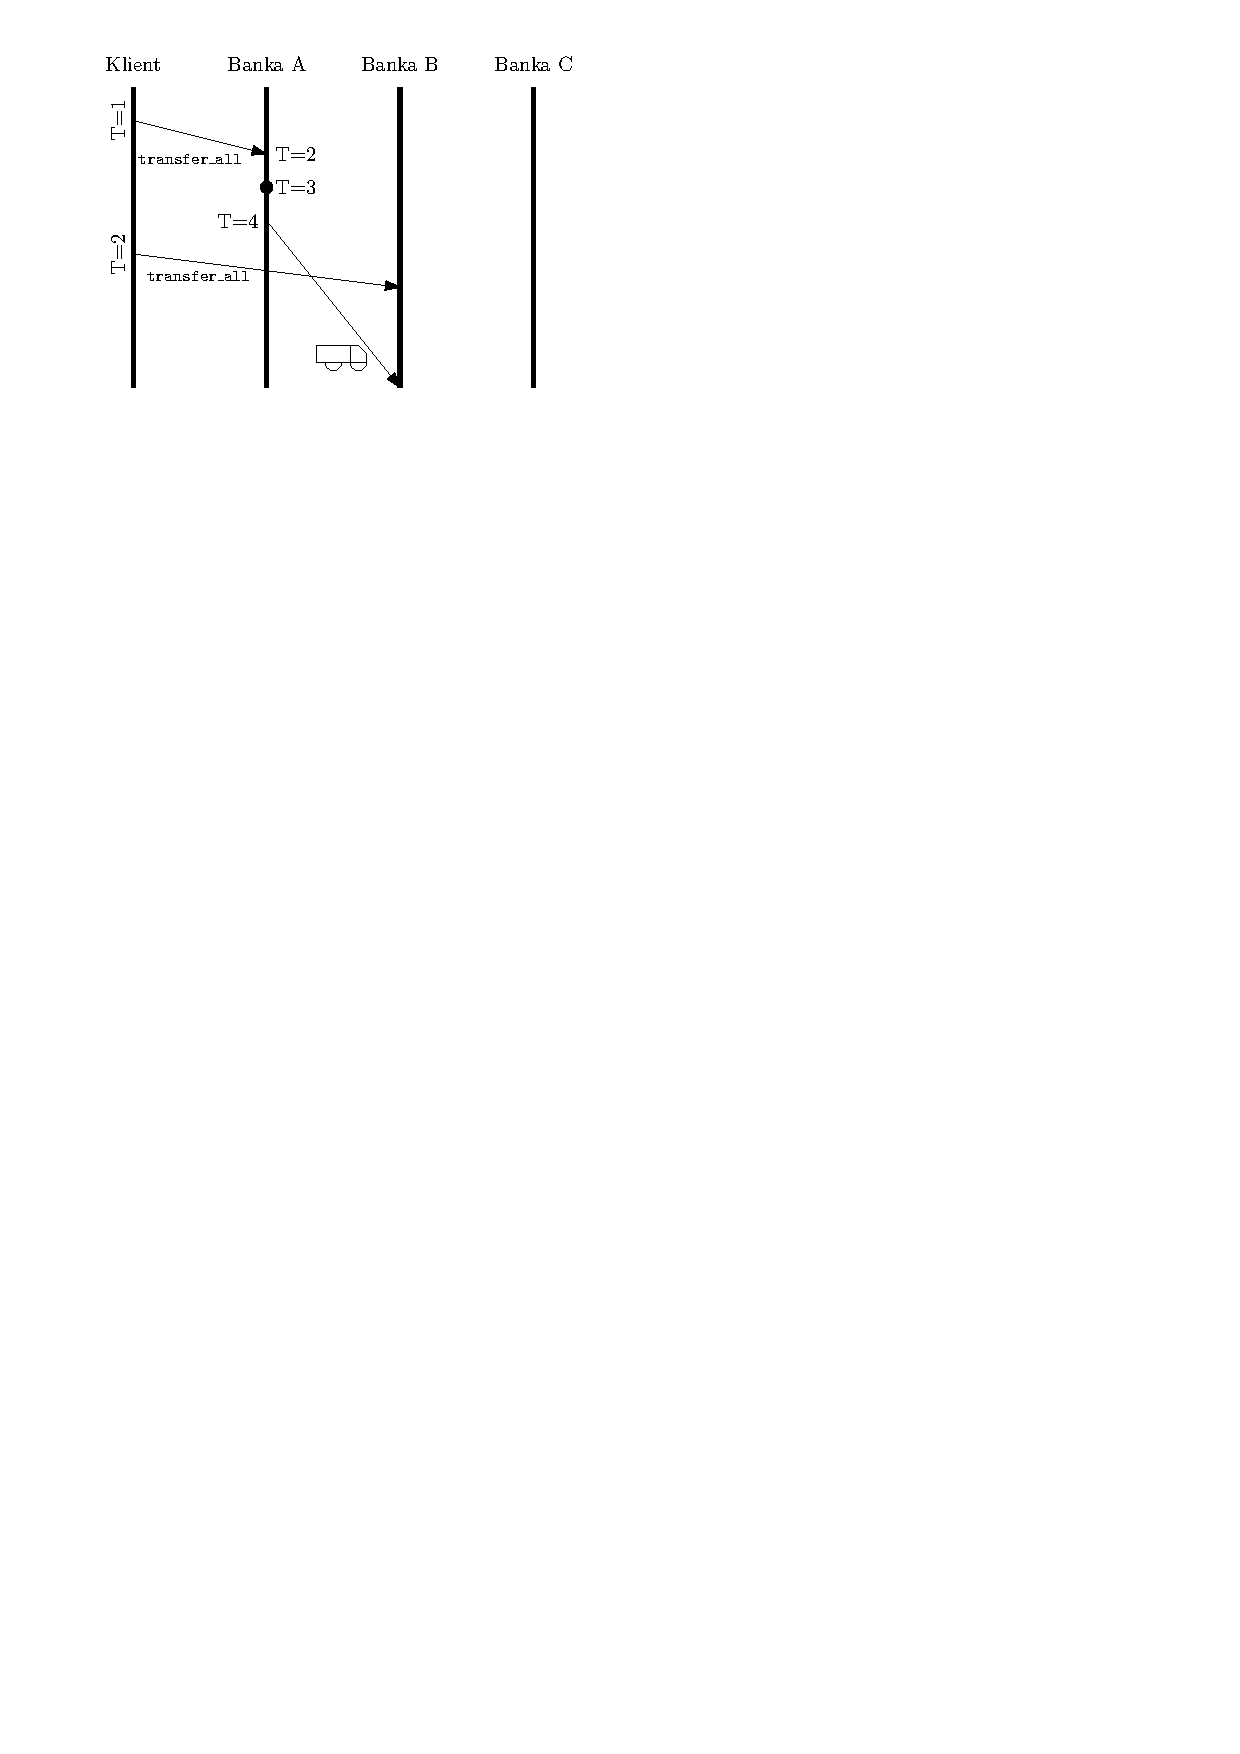
\includegraphics{10/figs/bank6.pdf}}%
%   	\only<7>{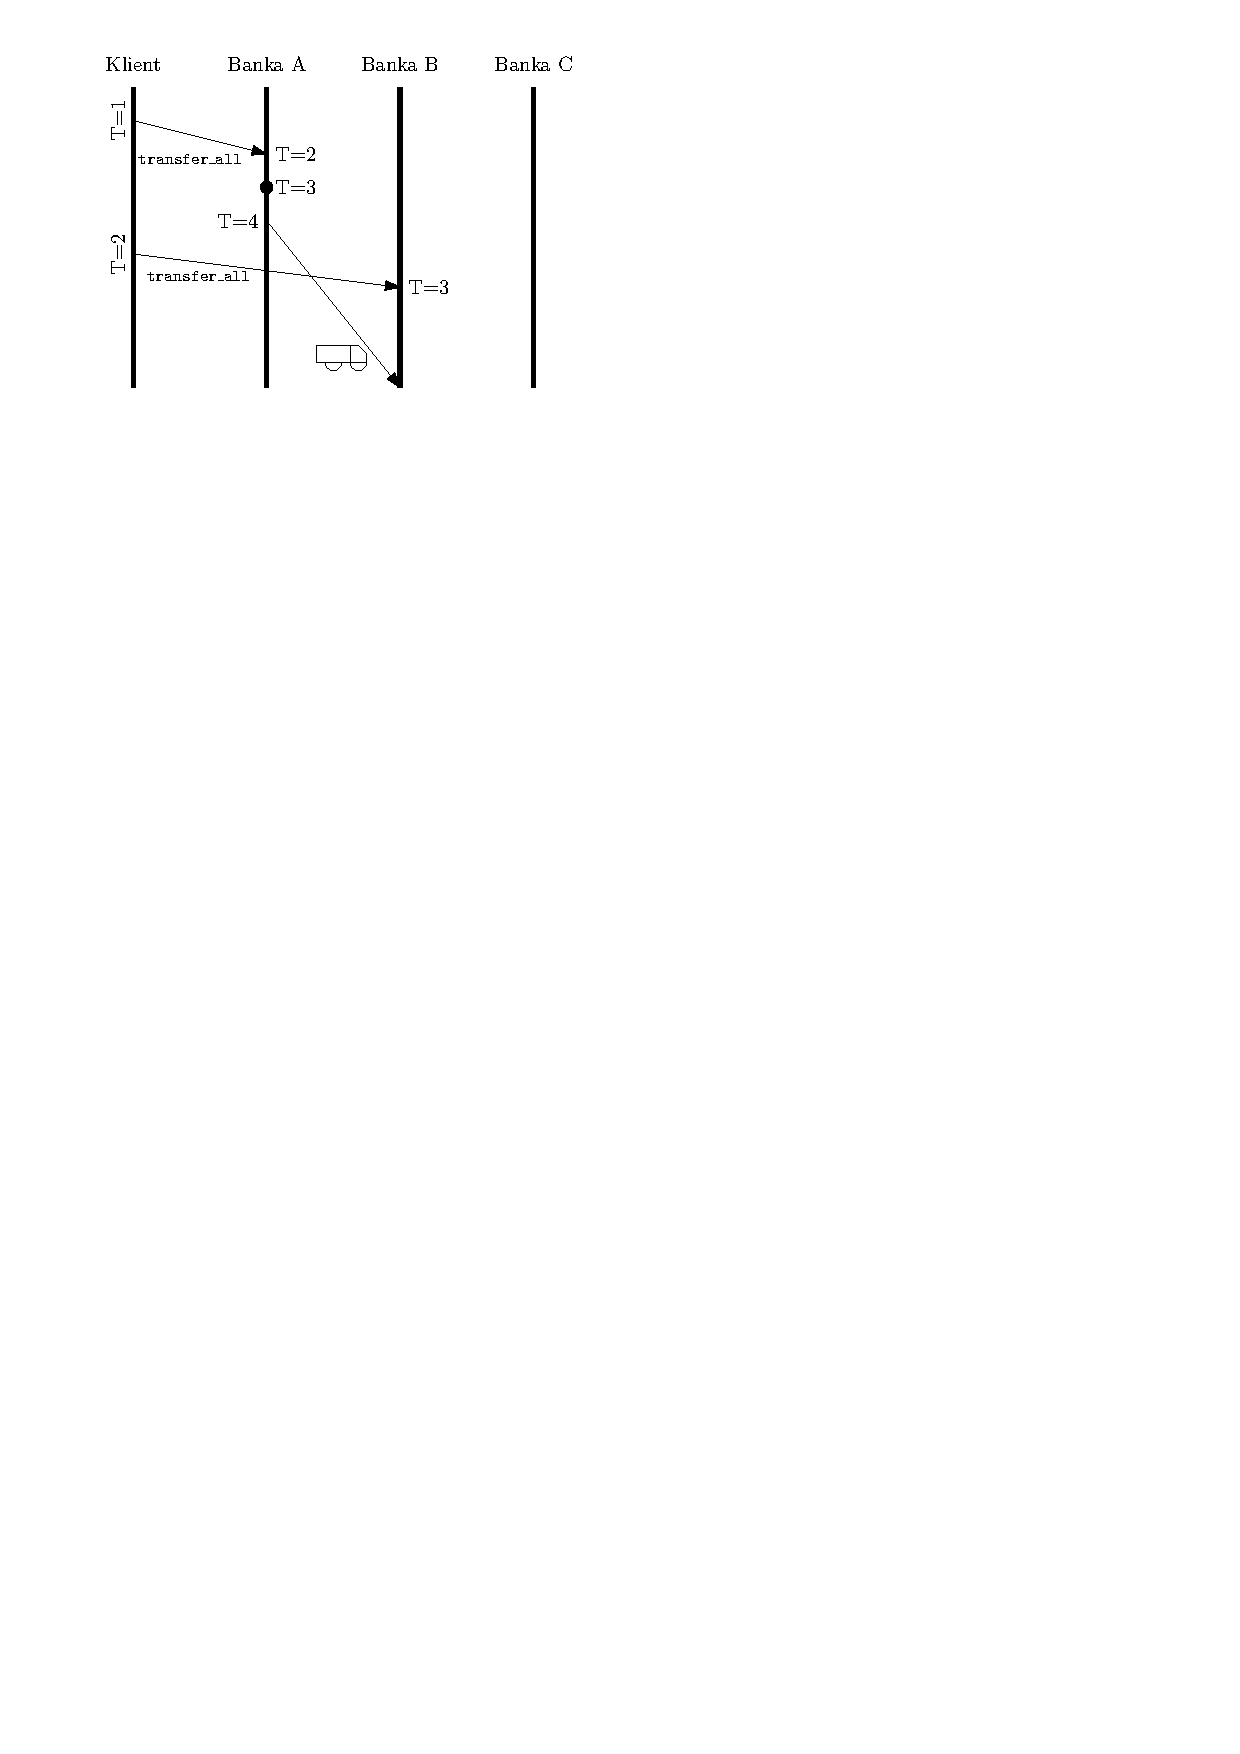
\includegraphics{10/figs/bank7.pdf}}%
%   	\only<8>{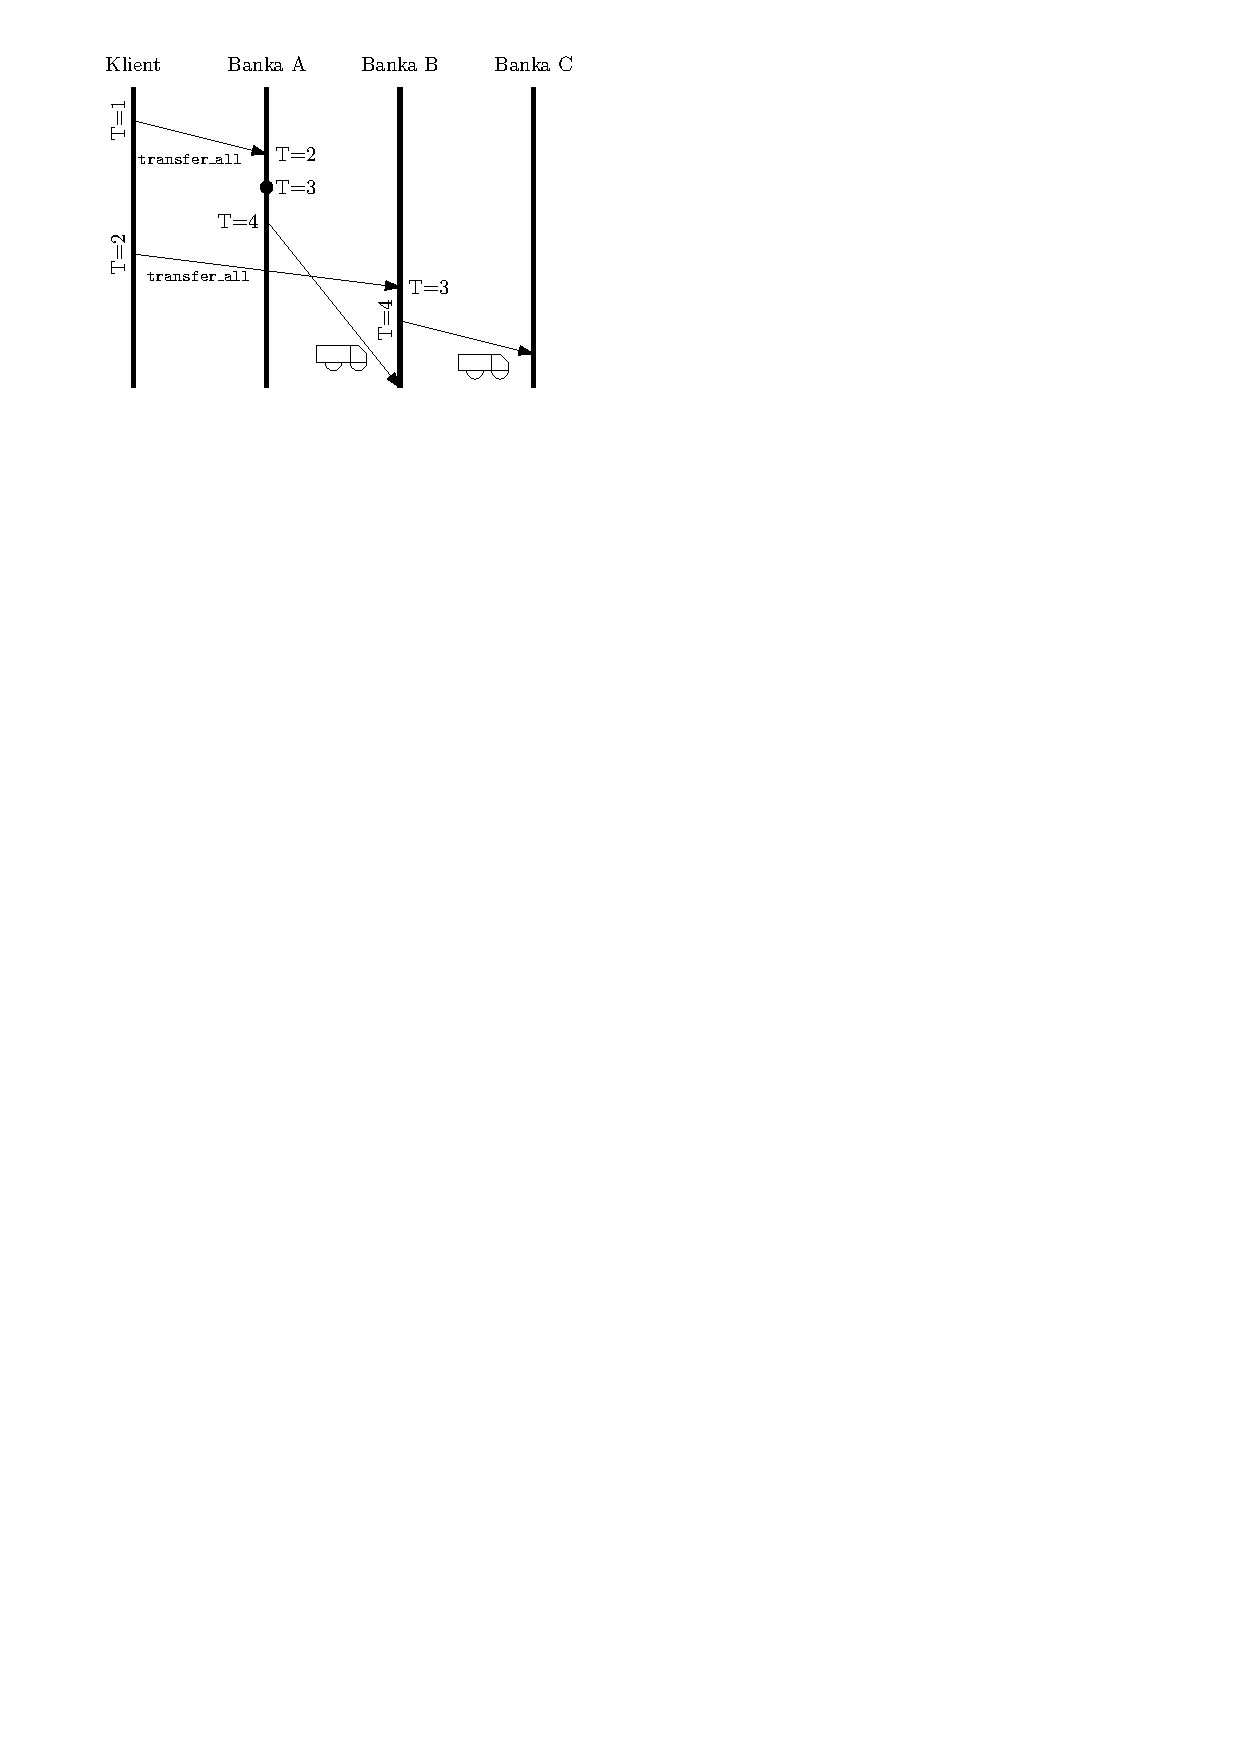
\includegraphics{10/figs/bank8.pdf}}%
%   	\only<9->{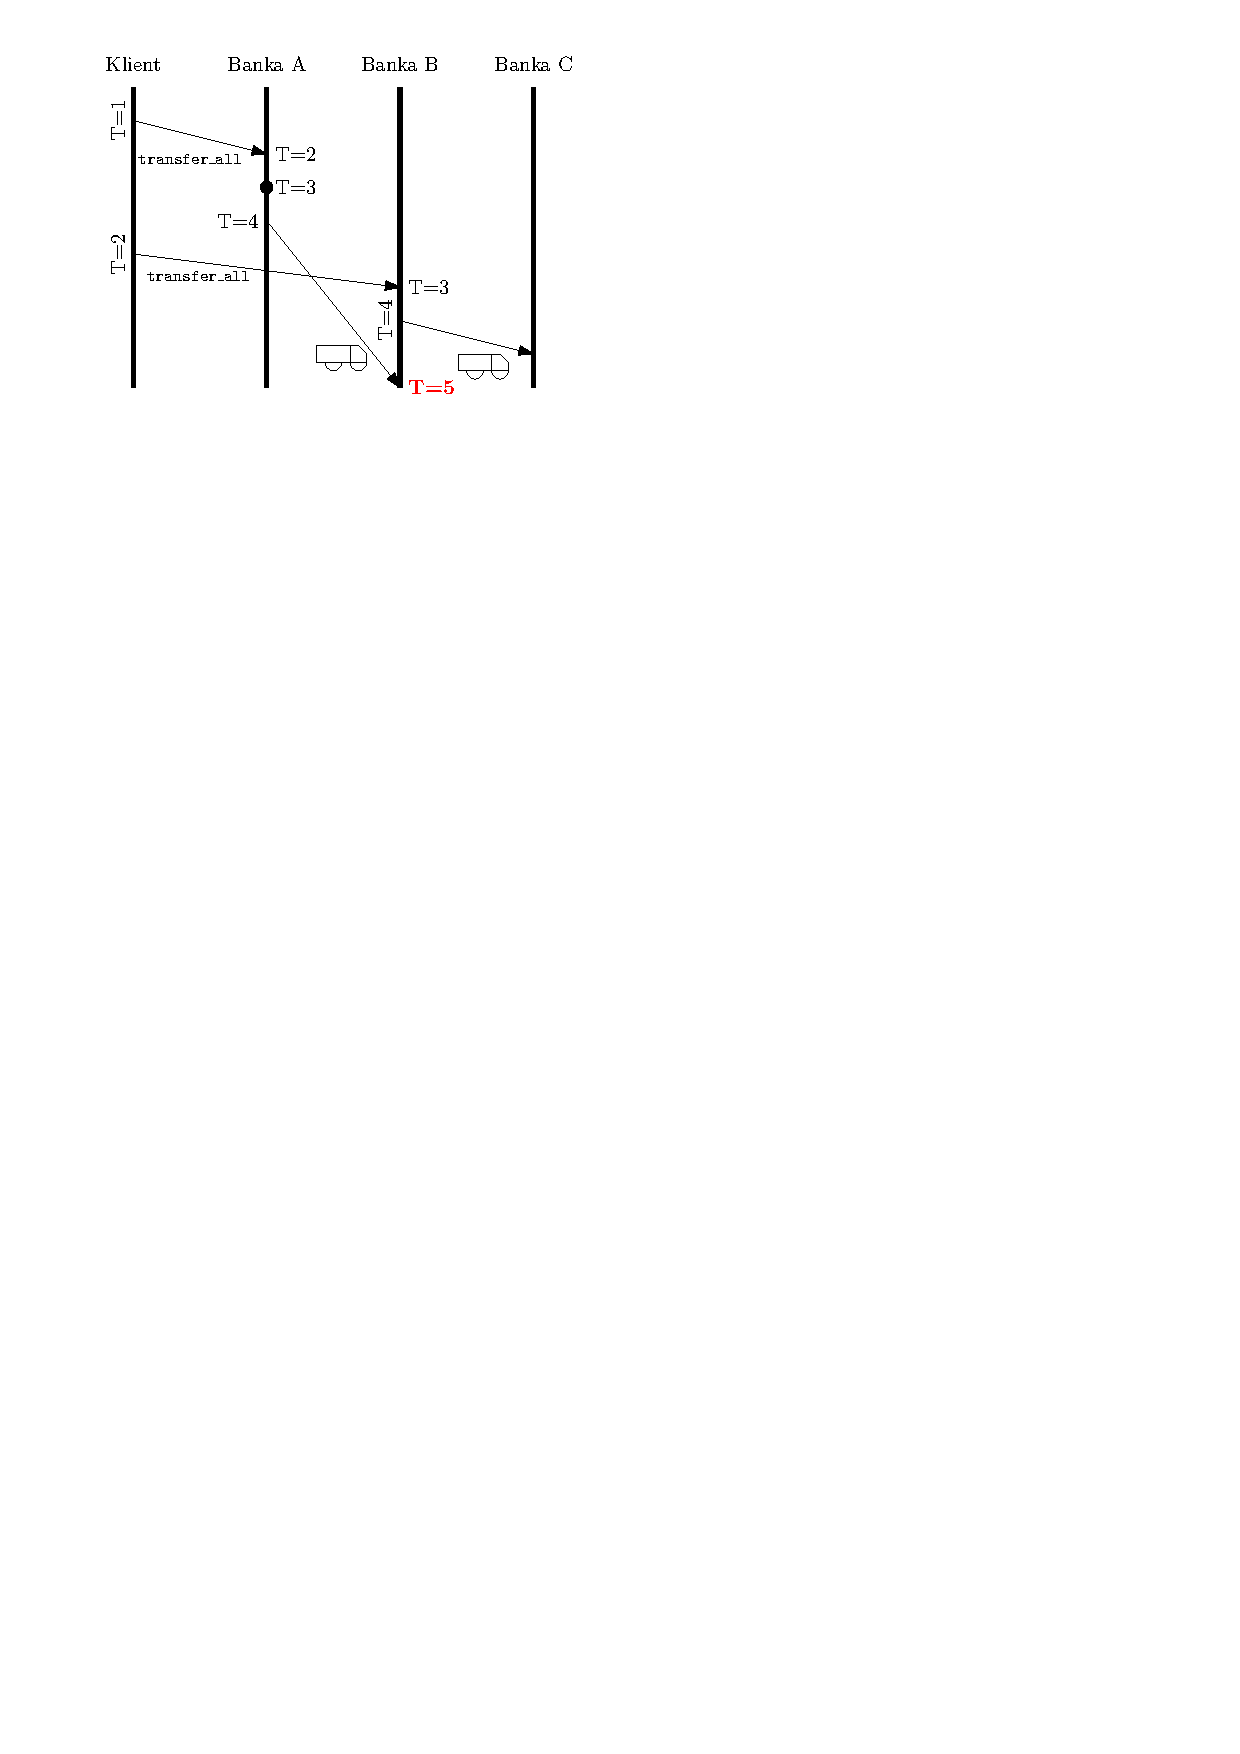
\includegraphics{10/figs/bank9.pdf}}%
%   \end{center}

%   \only<10>{
%   	\begin{center}
%   		\Large Skalární hodiny agregují všechny události do \underline{jediného} čísla :-(
%   	\end{center}
%   }
% \end{frame}

% \begin{frame}
%   \frametitle{Vektorové logické hodiny}

%   \begin{center}
%     \LARGE \bf Vektorové hodiny
%   \end{center}

%   \vspace{1em}\hrule\vspace{1em}

%   \begin{enumerate}
%     \pause\item Místo jednoho čísla si držíme vektor časů jednotlivých agentů \\
%   	            \mintinline{java}{int[] vectorTime = new int[NUM_AGENTS]}
%   	\pause\item Před každou významnou událostí (obzvlášť posláním zprávy!) si proces $i$ lokální čas posune... \textbf{Ale jen svoji komponentu!} \\
%   				\mintinline{java}{++vectorTime[i]}
%   	\pause\item Každé zprávě přiřadíme časovou značku $\texttt{msg.}T = \texttt{vectorTime}$
%   	\pause\item Po přijetí zprávy \texttt{msg} procesem $i$ si proces $i$ aktualizuje svůj \texttt{logicalTime}:
%   				\[ \texttt{vectorTime[j]} = \begin{cases}
%   				      1 + \max \lbrace \texttt{vectorTime[j]},\ \texttt{msg.}T\texttt{[j]} \rbrace & \text{if } i = j \\
%   				      \max \lbrace \texttt{vectorTime[j]},\ \texttt{msg.}T\texttt{[j]} \rbrace & \text{jinak}
%   				   \end{cases}
%   				\]
%   \end{enumerate}

%   \pause
%   \begin{center}
%   	\bf \faWarning \hspace{3pt} Vždy posunujeme jen svoji složku časového vektoru!
%   \end{center}

  %As with Lamport logical time each host maintains its own notion of the local time and updates it using the timestamps placed by the sender onto messages. But with vector logical time, the time contains more information -- it contains a vector representing the state of each host. In other words, this vector not only contains the event count for the host, itself, it also contains the last-known event counts on each and every other host.

  %Below is a summary of the rules for vector logical clocks:

  %Instead of just keeping our logical time, we keep a vector, V[], such that V[i] represents what we know of the logical time on processor i.
  %V[our_id] is our logical time
  %Send V[] vector with each message
  %On receive, merge both vectors, selecting the greater of the corresponding elements from each. Then increment the component for self. The event is said to have happened at new (incremented) time.
  %On send, increment time component for self. Send the updated timestamp vector with the message. The event is said to have happened at new (incremented) time.

% \end{frame}


% {\setbeamertemplate{frame footer}{\see{{\tt VectorClock.java} a {\tt VectorTimestamp.java}\sep{\tt Run VectorClockRun.java} v balíčku {\tt pdv\_cloud.vector}}}
% \begin{frame}

%   \begin{block}{Doprogramujte vektorové logické hodiny}
%     Doimplementujte logiku vektorových logických hodin ve třídě \texttt{VectorClock.java}. Následně spusťte scénář \texttt{VectorClockRun.java}.
%   \end{block}

%   \pause\faWarning \hspace{3pt}
%     \textbf{Jak využít vektorové logické hodiny k detekci souběžných událostí?}.

% \end{frame}
% }

% \begin{frame}
%   \begin{center}
%     \LARGE Jak protokol upravit, aby v nedocházelo k porušení kauzality?
%   \end{center}

%   \pause\vspace{1em}\hrule\vspace{1em}
%   Možností je mnoho, například:
%   \begin{itemize}
%     \pause\item Před odesláním \texttt{REFRESH} zprávy si počkat na potvrzení od databáze \\
%                 {\small (Odeslání \texttt{REFRESH} zprávy je kauzálním následkem úspěšné replikace)}
%     \pause\item Pozdržet vyhodnocení dotazu do doby, než replikace proběhne \\
%                 {\small (Druhému uživateli můžeme poslat, že má požadovat data zapsaná nejdříve v daném logickém čase)}
%   \end{itemize}
%   %Very shortly, we'll talk about designing a communication mechanism that avoid causality violations.
%   \pause
%   \begin{itemize}
%     \item[\faWarning] \bf Obecně chceme, aby události $e_1$, $e_2$, které mají proběhnout po sobě (tj. například čtení až po replikaci) byly ve vztahu kauzální závislosti.
%   \end{itemize}
% \end{frame}

\section{Zadání domácí úlohy}

\begin{frame}
  \frametitle{SWIM detektor}
  \begin{center}
  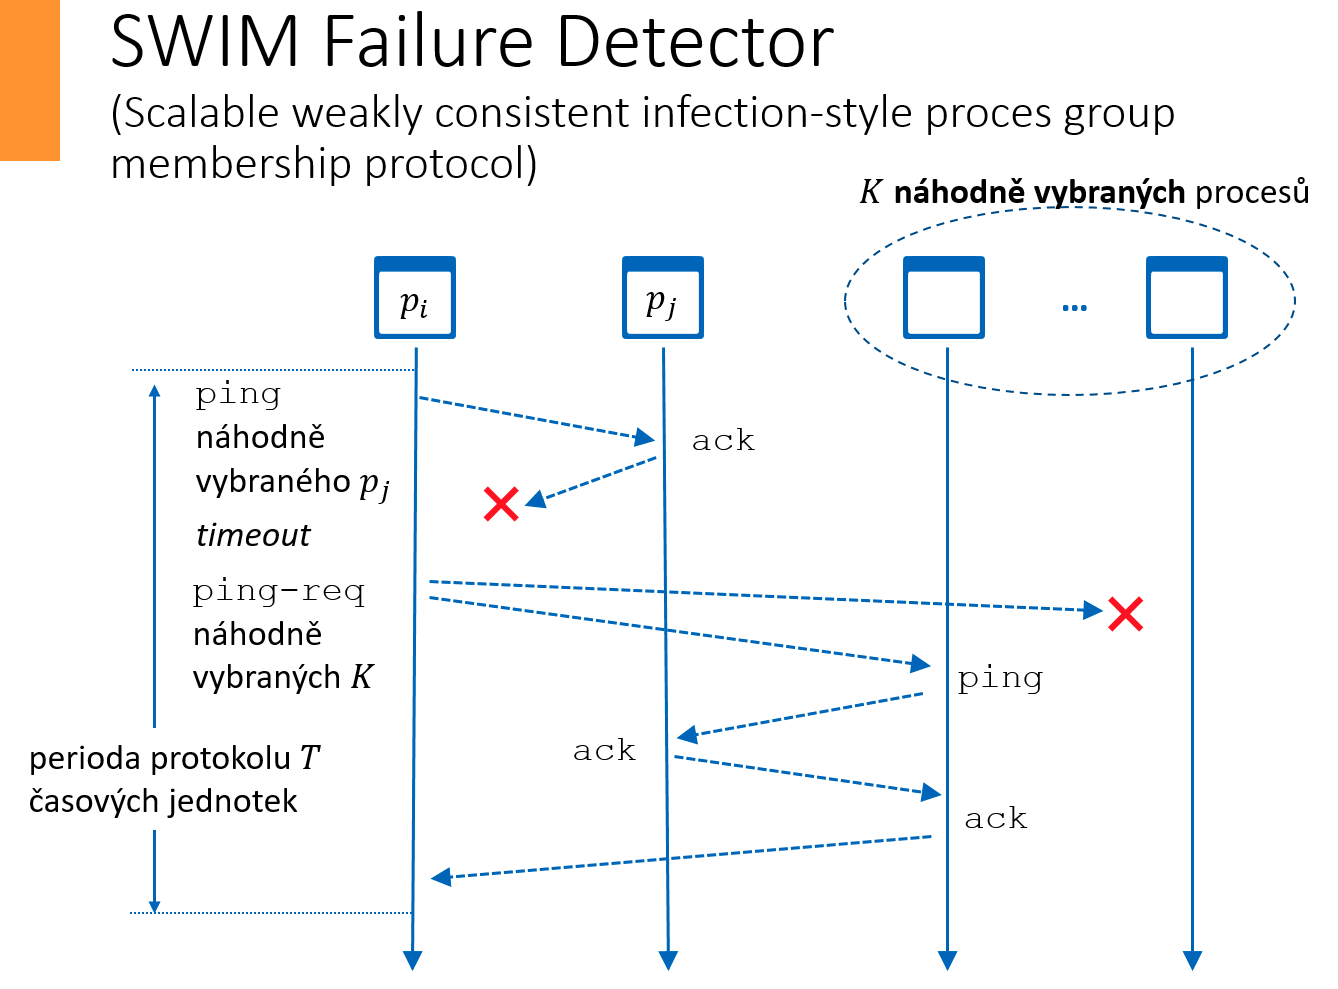
\includegraphics[width=\linewidth]{10/figs/swim.png}
  \end{center}
\end{frame}

\begin{frame}
  \frametitle{Distribuovaná databáze na komoditních serverech}
  \begin{center}
  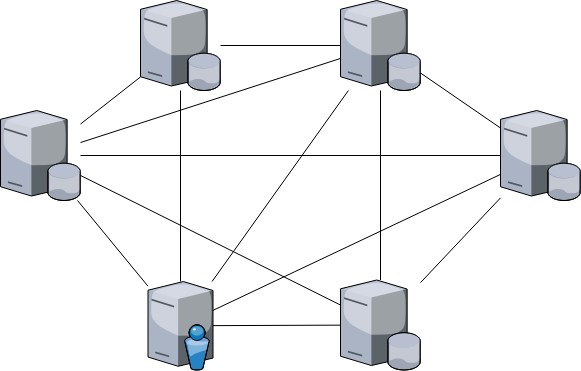
\includegraphics[width=.95\linewidth]{10/figs/dist_db.png}
  \end{center}
\end{frame}


\begin{frame}
  \frametitle{Distribuovaná databáze na komoditních serverech}
  Naimplementujte SWIM detekci selhání a zajistěte, že
  \begin{enumerate}
    \item zbytečně nevytěžuje síť;
    \item detekuje všechny ``mrtvé'' procesy s rozumnou rychlostí; a
    \item je dostatečně přesné.
  \end{enumerate}

  Zpracování musí být {\bf distribuované}, procesy si nesahají vzájemně do paměti!


%    \pause\vspace{1.5em}

%  \begin{tabbing}
%  Termín odevzdání je \={\bf 3.5. 23:59 CET} pro středeční cvičení a\\
%  \>{\bf 4.5. 23:59 CET} pro čtvrteční cvičení.
%\end{tabbing}

%\raggedleft Podrobnosti upřesníme.


\end{frame}


% Frame with the feedback QR code
\framefeedback{}

\end{document}
